\chapter{Medical Devices: Current State and Challenges}

The medical device market is worth \$289 billion, of which \$110 billion is from the US alone, with this number projected to reach \$133 billion in 2016 (\cite{market1}).
Examples include everything from adhesive bandages, stents, artificial joints, drug infusion pumps to surgical robots, implantable cardiac pacemakers, and devices still undergoing basic research like the artificial pancreas.
To take one example of the societal impact of medical devices, an estimated 3 million people worldwide have implanted cardiac pacemakers (a heart rate management device), with 600,000 added annually.
Clinical trials have presented evidence that patients implanted with cardiac defibrillators (another heart rate management device) have a mortality rate reduced by up to 31\% (\cite{maditrit}).
% MADIT II trial

%With the increasing complexity of combining hardware and software in a large class of these life-saving technologies, there is an urgent need for approaches to rigorously validate the device and therapy to be safe and efficacious.
\begin{figure}[t]
		\centering
		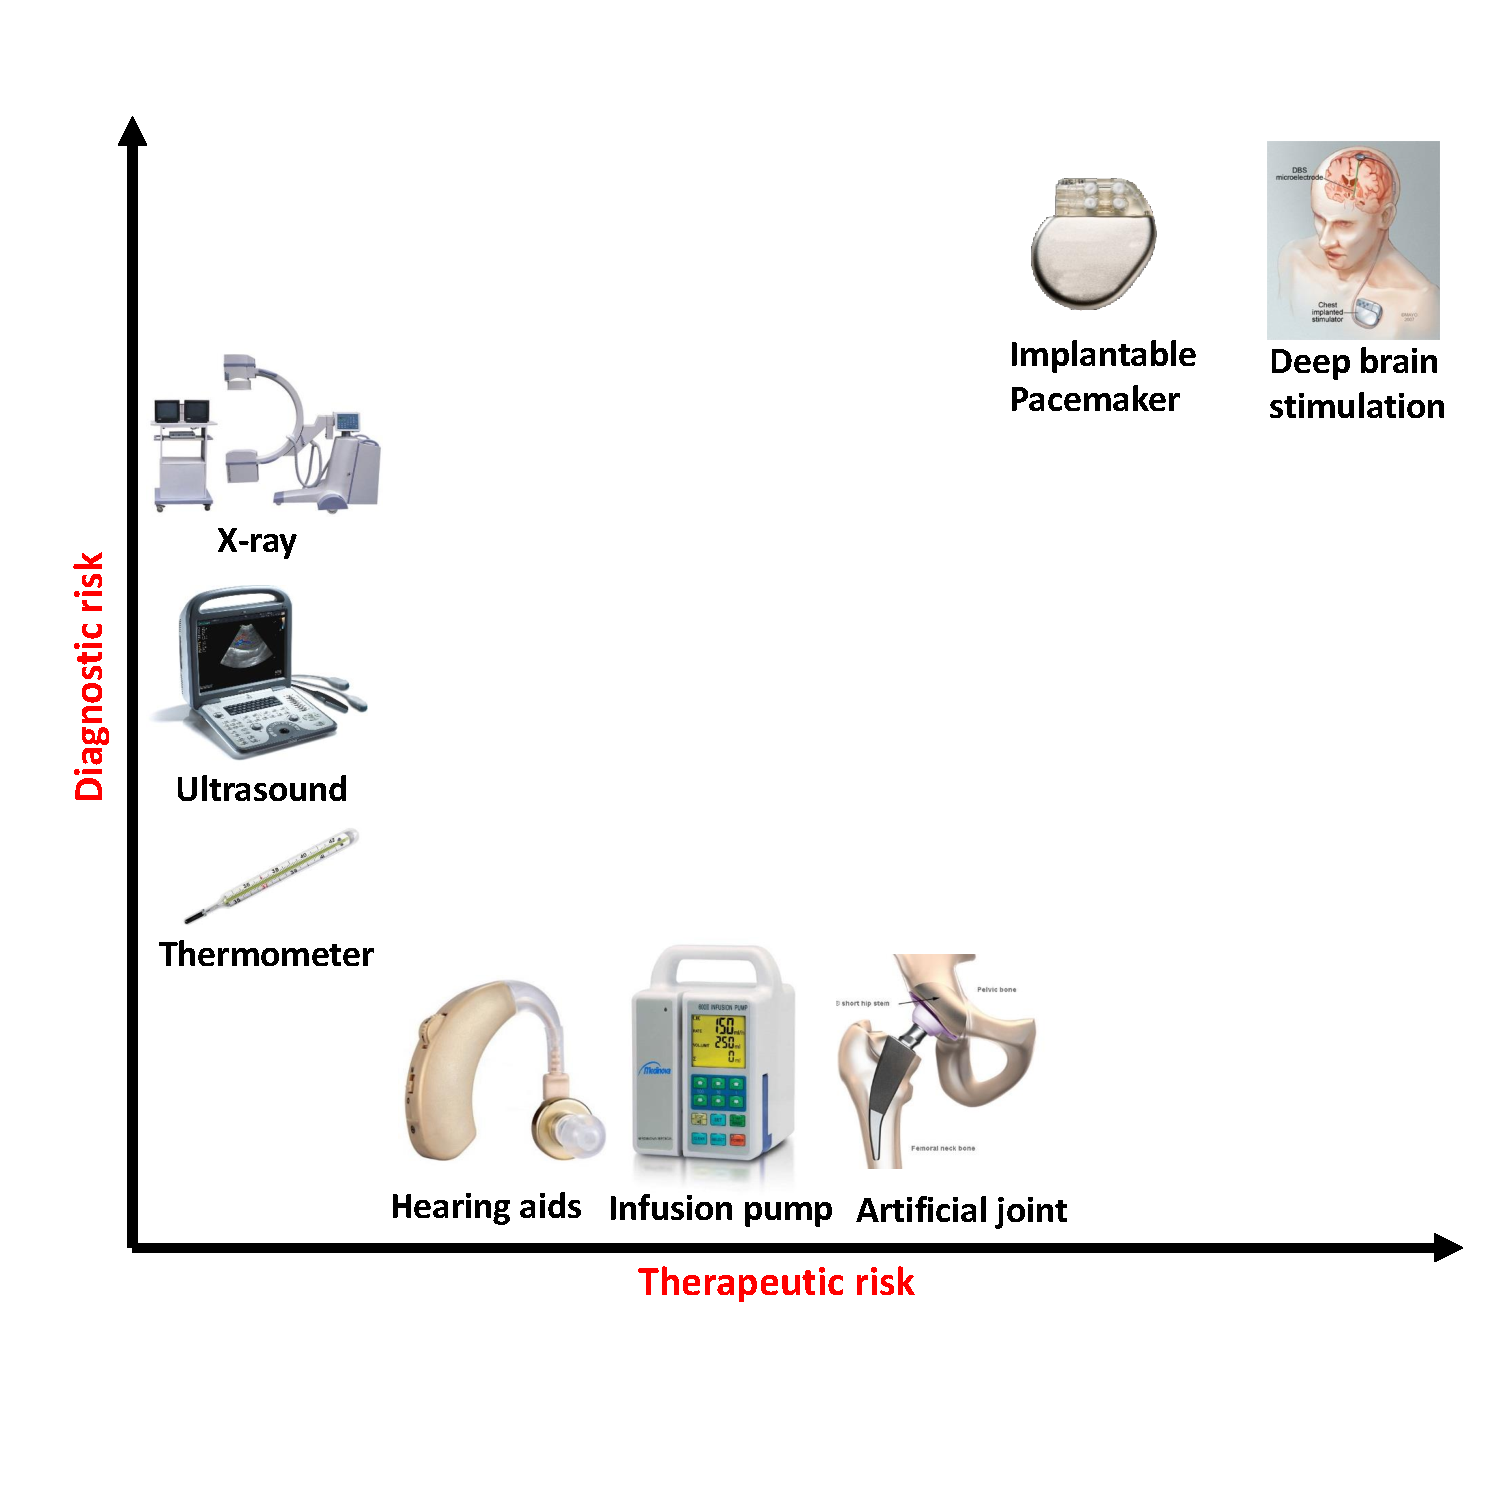
\includegraphics[width=\textwidth]{figs/devices_new.pdf}
		\caption{\small Current medical devices across a range of diagnostic and therapeutic risk. Implantable software-controlled devices such as the pacemaker and defibrillator which operate in a closed-loop of sensing, control and actuation are amongst the highest risk}
		\label{fig:Cur}
\end{figure}

The US Food and Drug Administration (FDA) defines a medical device as an instrument, apparatus, implement, machine, or implant which is:
\begin{itemize}
	\item intended for use in the diagnosis of disease or other conditions, or in the cure, mitigation, treatment, or prevention of disease, in humans or other animals, or
	\item intended to affect the structure or any function of the human body or other animals, and which does not achieve any of its primary intended purposes through chemical action and which is not dependent upon being metabolized for the achievement of any of its primary intended purposes."
\end{itemize}

In general, medical devices are categorized according to their risk factors - Class I, Class II and Class III, corresponding to low-risk, medium-risk and high-risk devices (\cite{class}).  
\figref{Cur} gives an intuitive description of medical devices examples across a range of diagnostic and therapeutic risk.

\begin{figure}[t]
		\centering
		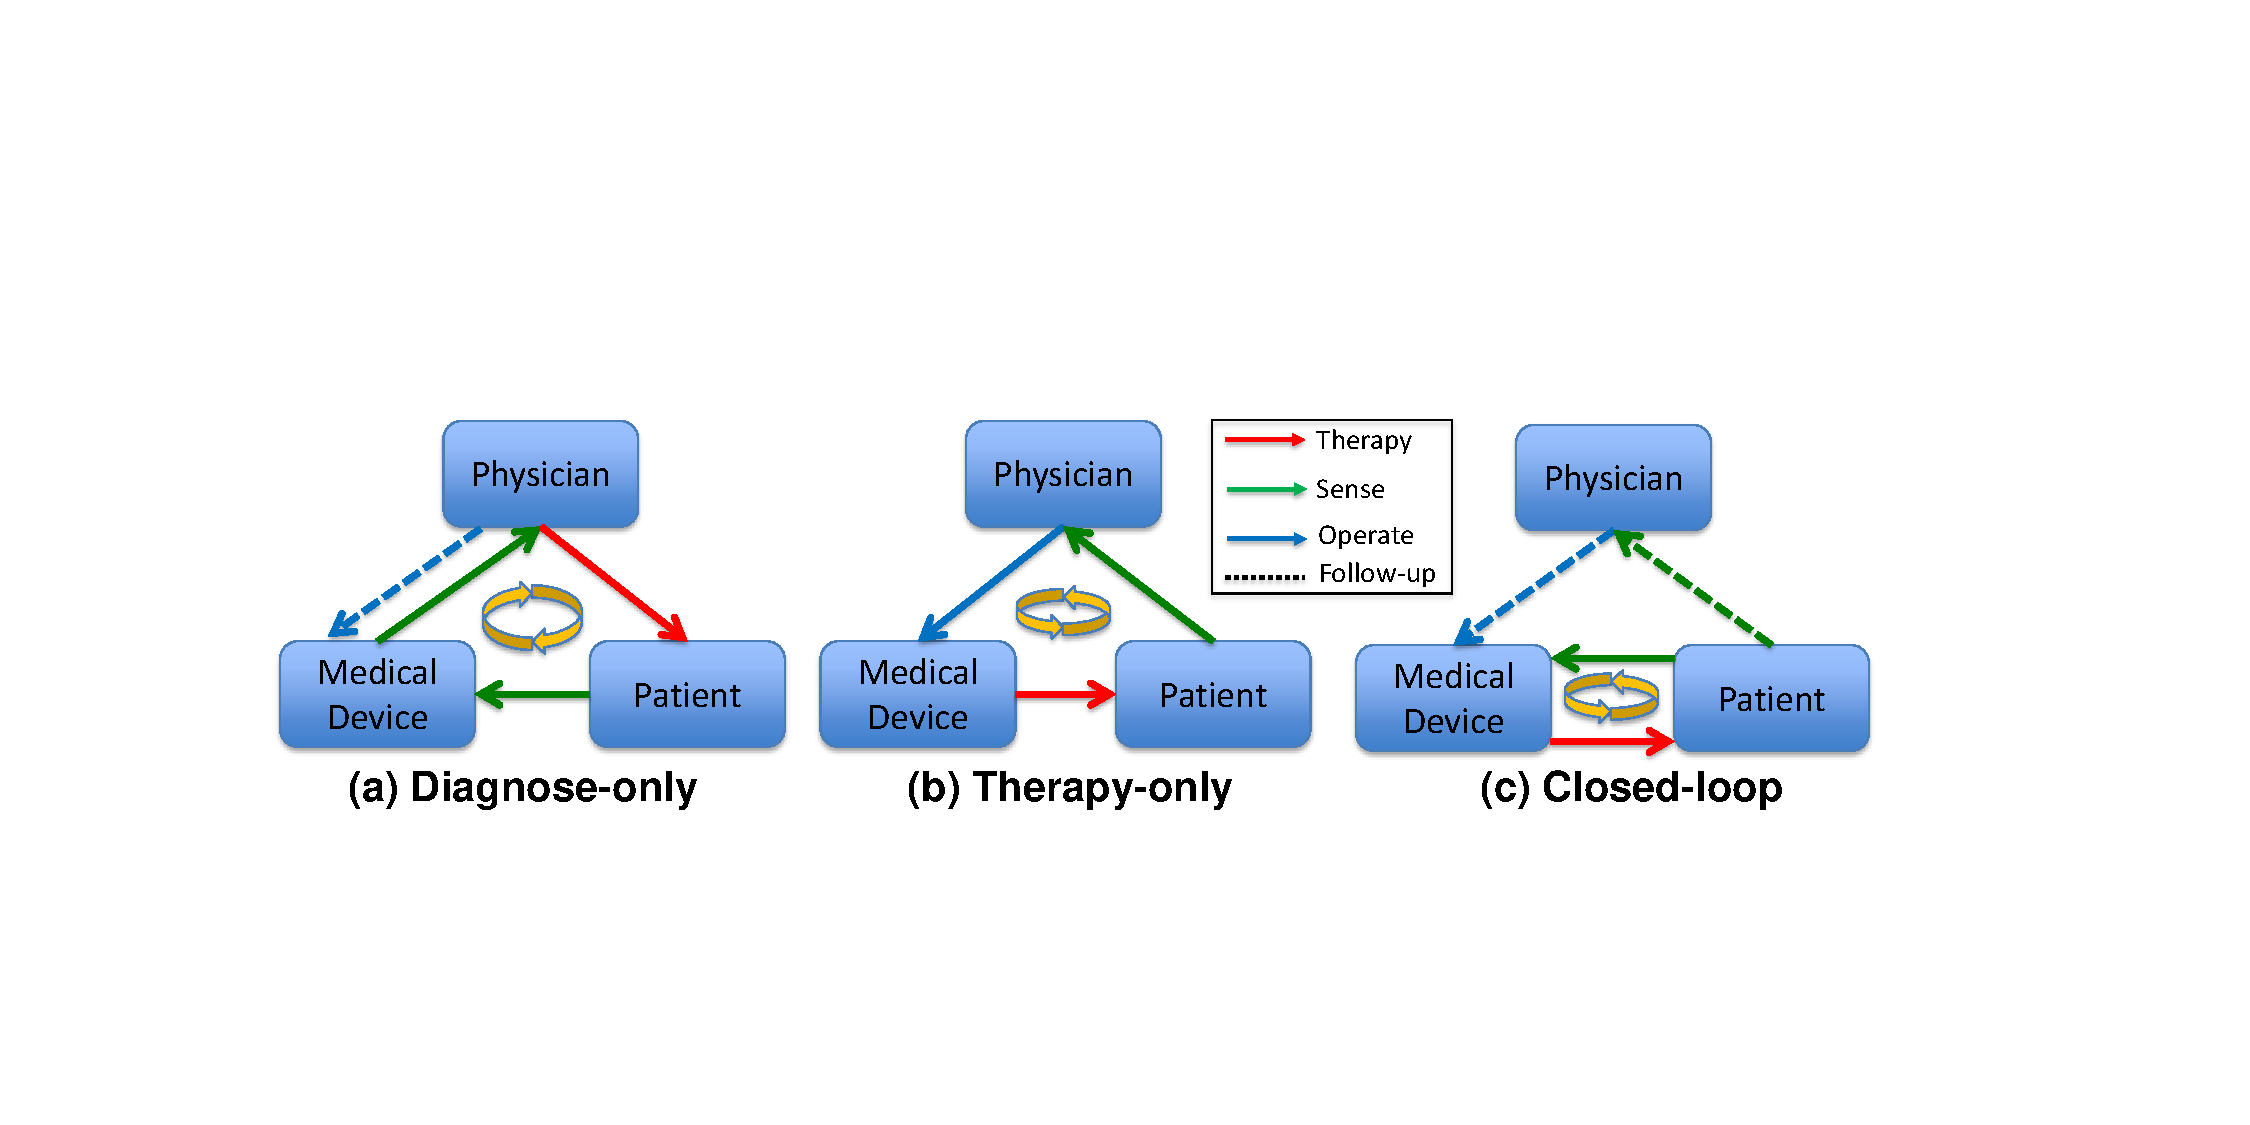
\includegraphics[width=\textwidth]{figs/closed-loop.pdf}
		\caption{\small Diagnostic-only and therapy-only devices do not interact with the patient in direct closed-loop. The physician is responsible for the diagnostic and/or therapeutic decisions. However in closed-loop medical devices, the devices interact with the patient in closed-loop and have to make therapeutic decisions based on their own diagnosis.}
		\label{fig:closed-loop}
\end{figure}

\section{Closing the Device-Patient Loop}
Medical devices operate across a range of invasiveness and intervention with the patient in the loop. 
For diagnostic-only devices, like an X-ray machine, the medical professional operates the device to obtain patient data. 
Upon interpretation of the data, the medical professional performs diagnosis followed by delivery of proper therapy to the patient (\figref{closed-loop}.(a)). 
For therapy-only devices, e.g. a drug infusion pump, the medical professional configures the device infrequently based on prior diagnosis of the patient so the device only executes the therapy on the patient (\figref{closed-loop}.(b)). 
We denote these devices as \textbf{Open-loop Medical Devices} as there is no direct feedback between the patient and the device. 
For open-loop devices, the device operates under the supervision of professionally-trained physicians. 
The device's safety is mostly determined by how accurately it provides information to the physicians or how faithfully it operates as instructed by the physicians.

There is a class of devices with both diagnostic and therapeutic functions, i.e. implantable cardiac devices to treat cardiac arrhythmia, deep brain stimulation devices (\cite{Brain_sti}) to treat Parkinson's disease and artificial pancreas to treat Type-1 diabetes. 
These devices capture and diagnose the patient's physiological conditions from patient signals, \emph{and} deliver therapy in response (\figref{closed-loop}.(c)). These devices usually operate autonomously with very little human intervention. 
We denote them as \textbf{Autonomous Medical Devices}. 
The benefits of autonomous medical devices are timely therapy and more independent life-style.
However, autonomy of these medical devices also brings about safety and efficacy concerns. 
%Malfunctions or inappropriate therapies from these devices also cannot be corrected timely, which can cause serious adverse effects on patients' health. 
With open-loop medical devices, the diagnosis and therapy decisions are made by medical professionals, who have expert knowledge of human physiology. 
Therefore they are able to identify adverse health conditions and adjust the therapy accordingly. 
On the other hand, closed-loop medical devices have to make both the diagnosis and therapy decisions on their own. 
The domain expertise required to make those decisions has to be programmed into the device. 
It is not feasible to encode all the knowledge of human physiology into the device. 
For unanticipated physiological conditions, when the appropriate response has not been programmed into the device, the device may deliver inappropriate therapy which can have an adverse effect on patient's health. 
Therefore, these devices are usually classified into the highest risk category and undergo the most stringent regulation. 
\subsection{Challenges for Developing Autonomous medical Devices}
There are multiple challenges to develop safe and effective autonomous medical devices:

\subsubsection{Physiological Complexity} 
Human physiology is complex and not completely understood. 
For instance, the functionality of the heart can be interpreted from \emph{multiple perspectives}: from its electrical activity, mechanical contractions of the heart muscles, and dynamics of blood flow. 
The physiology of the heart can also be analyzed with \emph{multiple scales}: from the molecular level to cellular level all the way to the organ and system level. 
It is impossible to encode all these contexts into the device, hence inappropriate diagnosis and therapy are observed due to the lack of physiological contexts (~\cite{killedbycode, icd_recall}).
	\subsubsection{Physiological Variability}
	Physiological conditions and parameters demonstrate different levels of variability both within the individual at different times, levels of exertion and under the influence of medication and also across individuals. 
	For instance, a segment of the population may have additional electrical conduction pathways within their heart, which makes them vulnerable to certain heart diseases.
	Consequently, autonomous medical devices should be able to safely operate under a large variety of physiological conditions. 
	This is difficult to guarantee, as the device designer must consider all possible physiological conditions, and their interaction with the device, during the development of the device.
	%\hatodoin{last sentence: rather than say "always", say something like: "the designer will likely miss some rare conditions during the design of the device".}
	
	\subsubsection{Limited Observability} 
	Autonomous medical devices normally rely on minimally invasive measurement of the physiological parameters in order to allow the patients to live their normal life. 
	For example, implantable pacemakers and defibrillators commonly have only two leads and therefore two points of observation for the whole heart. 
	The limited observability inevitably leads to ambiguities as different physiological conditions can map to the same input sequence to the device, resulting in inaccurate diagnosis and therapy. 

\subsubsection{Software-related Medical Device Recalls}
The diagnostic and therapeutic functions of the autonomous medical devices are mostly controlled by their software components due to their complexity. 
For instance, implanted cardiac pacemakers and defibrillators have approximately 80,000-100,000 lines of software code which essentially makes all sensing, control and actuation decisions autonomously within the human body, over the 5-7 year device lifetime \footnote{Paul L. Jones. Senior Systems/Software Engineer, Office of Science and Engineering Laboratories, U. S. FDA. Personal communication, 2010.}. 
Software embedded in a medical device, unlike electrical and mechanical components, does not fail due to corrosion, fatigue or have statistical failures of sub-components. 
Software failures are uniquely sourced in the design and development of the system. %Unlike other industries such as consumer electronics where product life cycles are measured in months, software engineering for medical devices often spans a decade and must prioritize safety and efficacy over time to market. 
%\begin{figure}[t]
		%\centering
		%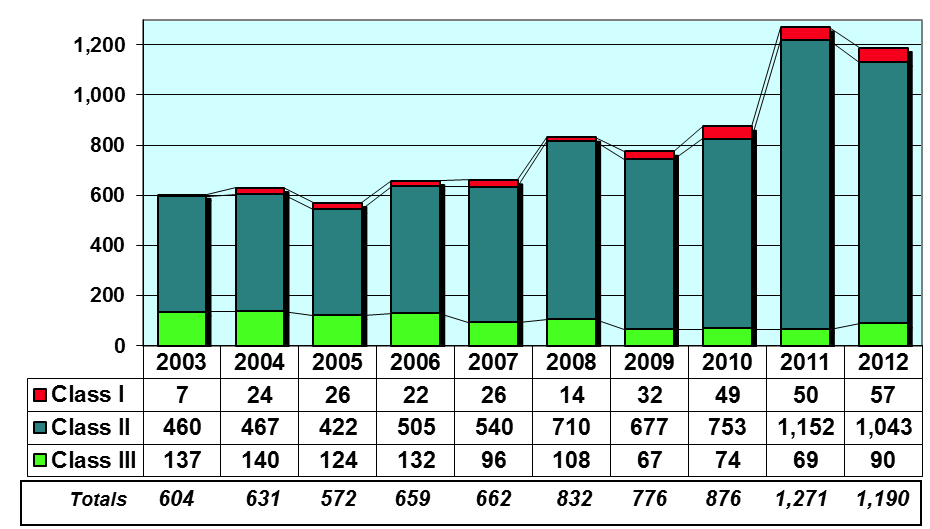
\includegraphics[width=0.8\textwidth]{figs/recalls.jpg}
		%\caption{\small Medical device recalls have risen over the past decade}
		%\label{fig:recalls}
%\end{figure}
\begin{figure}[t]
		\centering
		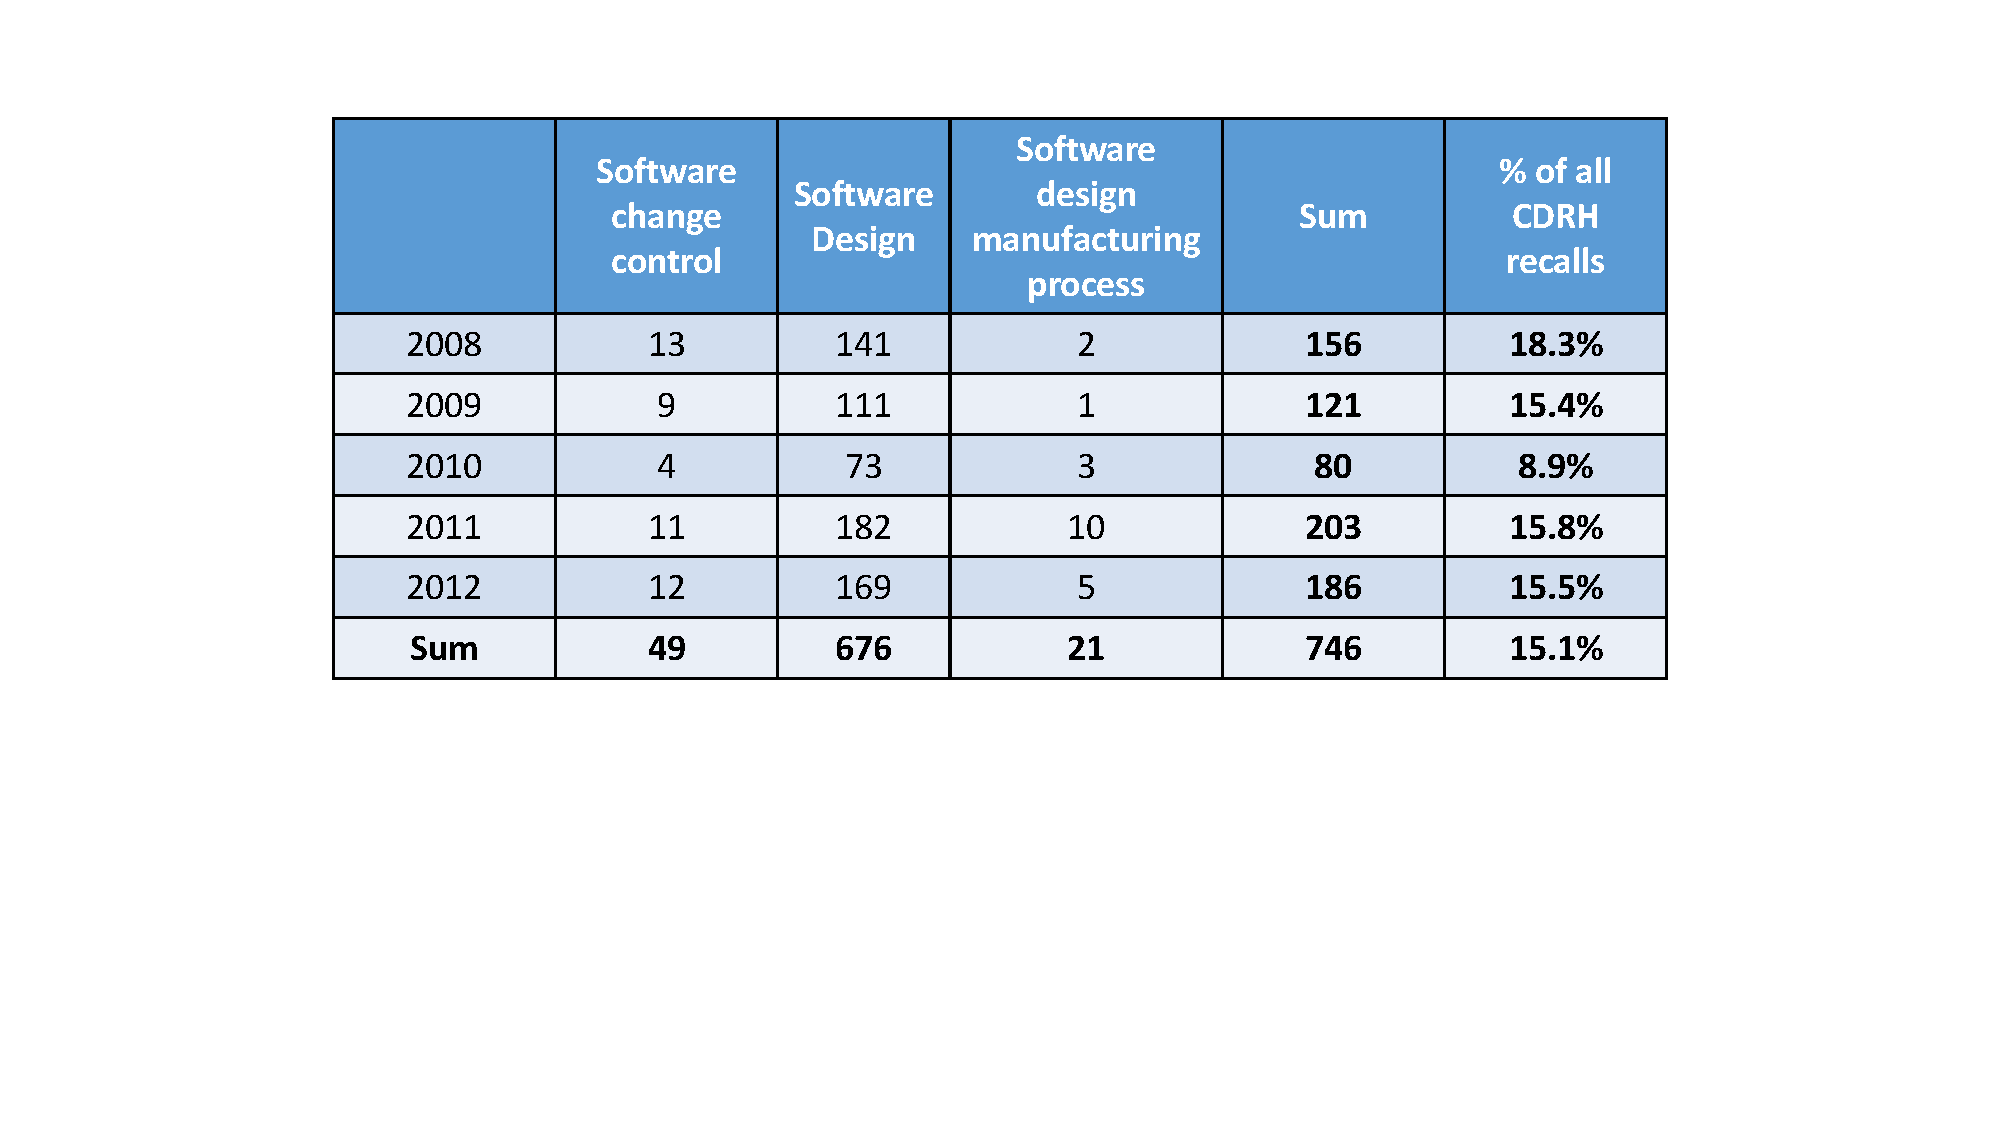
\includegraphics[width=0.8\textwidth]{figs/recalls.pdf}
		\caption{\small Medical device recalls due to software issues have risen from 10\% in the 1990s to \~15\% in the past decade (\cite{recall_rep})}
		\label{fig:soft_recalls}
\end{figure}
%  Over the course of the past four decades, cardiac rhythm management devices such as pacemakers and implantable cardioverter defibrillators (ICD) have grown in complexity and now have more than 80,000 to 100,000 lines of code (\cite{pauljones}). 

According to the US Food and Drug Administration, in 1996, 10\% of all medical device recalls were caused by software-related issues (\cite{medstats}). 
This percentage rose to an average of 15\% of recalls from 2008 to 2012 (\figref{soft_recalls}). 
Malfunctions of closed-loop medical devices usually have severe consequences, which will be categorized as \emph{Class I}, meaning there is a ``reasonable probability that use of these products will cause serious adverse health consequences or death.'' (\cite{medstats2,pacemakerrecalls,killedbycode}). 



\section{Medical Device Regulation Efforts and Challenges}
%The medical device industry is regulated to ensure the safety of the patients and the public. 
In the United States, the FDA is the primary regulatory authority responsible for assuring the \emph{safety, efficacy and security }of patients using medical devices. 
%These three terms can be further elaborated as:
%\begin{itemize}
	%\item \emph{Efficacy}: The device is effective in achieving its intended and expected use.
	%\item \emph{Safety}: The device does not expose the patient, user, or other bystanders to undue risk from its use;
	%\item \emph{Security}: The device has been designed to protect patients, users, and bystanders from both unintentional and malicious misuse of the device
%\end{itemize}
%\begin{itemize}
	%\item Efficacy: The device is effective in achieving its intended and expected use.
	%\item Safety: The device does not expose the patient, user, or other bystanders to undue risk from its use;
	%\item Security: The device has been designed to protect patients, users, and bystanders from both unintentional and malicious misuse of the device
%\end{itemize}
Based on the rationale that 1) manufacturers know their devices better than the regulator, and 2) the variety of medical devices requires a variety of approaches, it is the device manufacturers' responsibility to demonstrate the safety and efficacy of the medical devices. 
Manufacturers are required to complete a pre-market submission before the devices can be released to the market. 
The level of requirements for the submission is determined by the safety classification of the devices.

\subsection{Guidelines During Device Development}
A set of general guidelines are recommended by the FDA (\cite{fda1, fda2, fda3}) which list the activities that need to be performed during the development of the devices. 
In safety-critical industries such as automotive electronics, avionics and nuclear systems, international standards are \textbf{enforced} for software system development, evaluation, manufacturing and post-market changes (\cite{autosar,avsi}). 
This awareness is only beginning to enter the medical device industry as compliance with international standards are "recommended" in the aforementioned guidelines (\cite{formal_fda}). 

\begin{figure}[t]
		\centering
		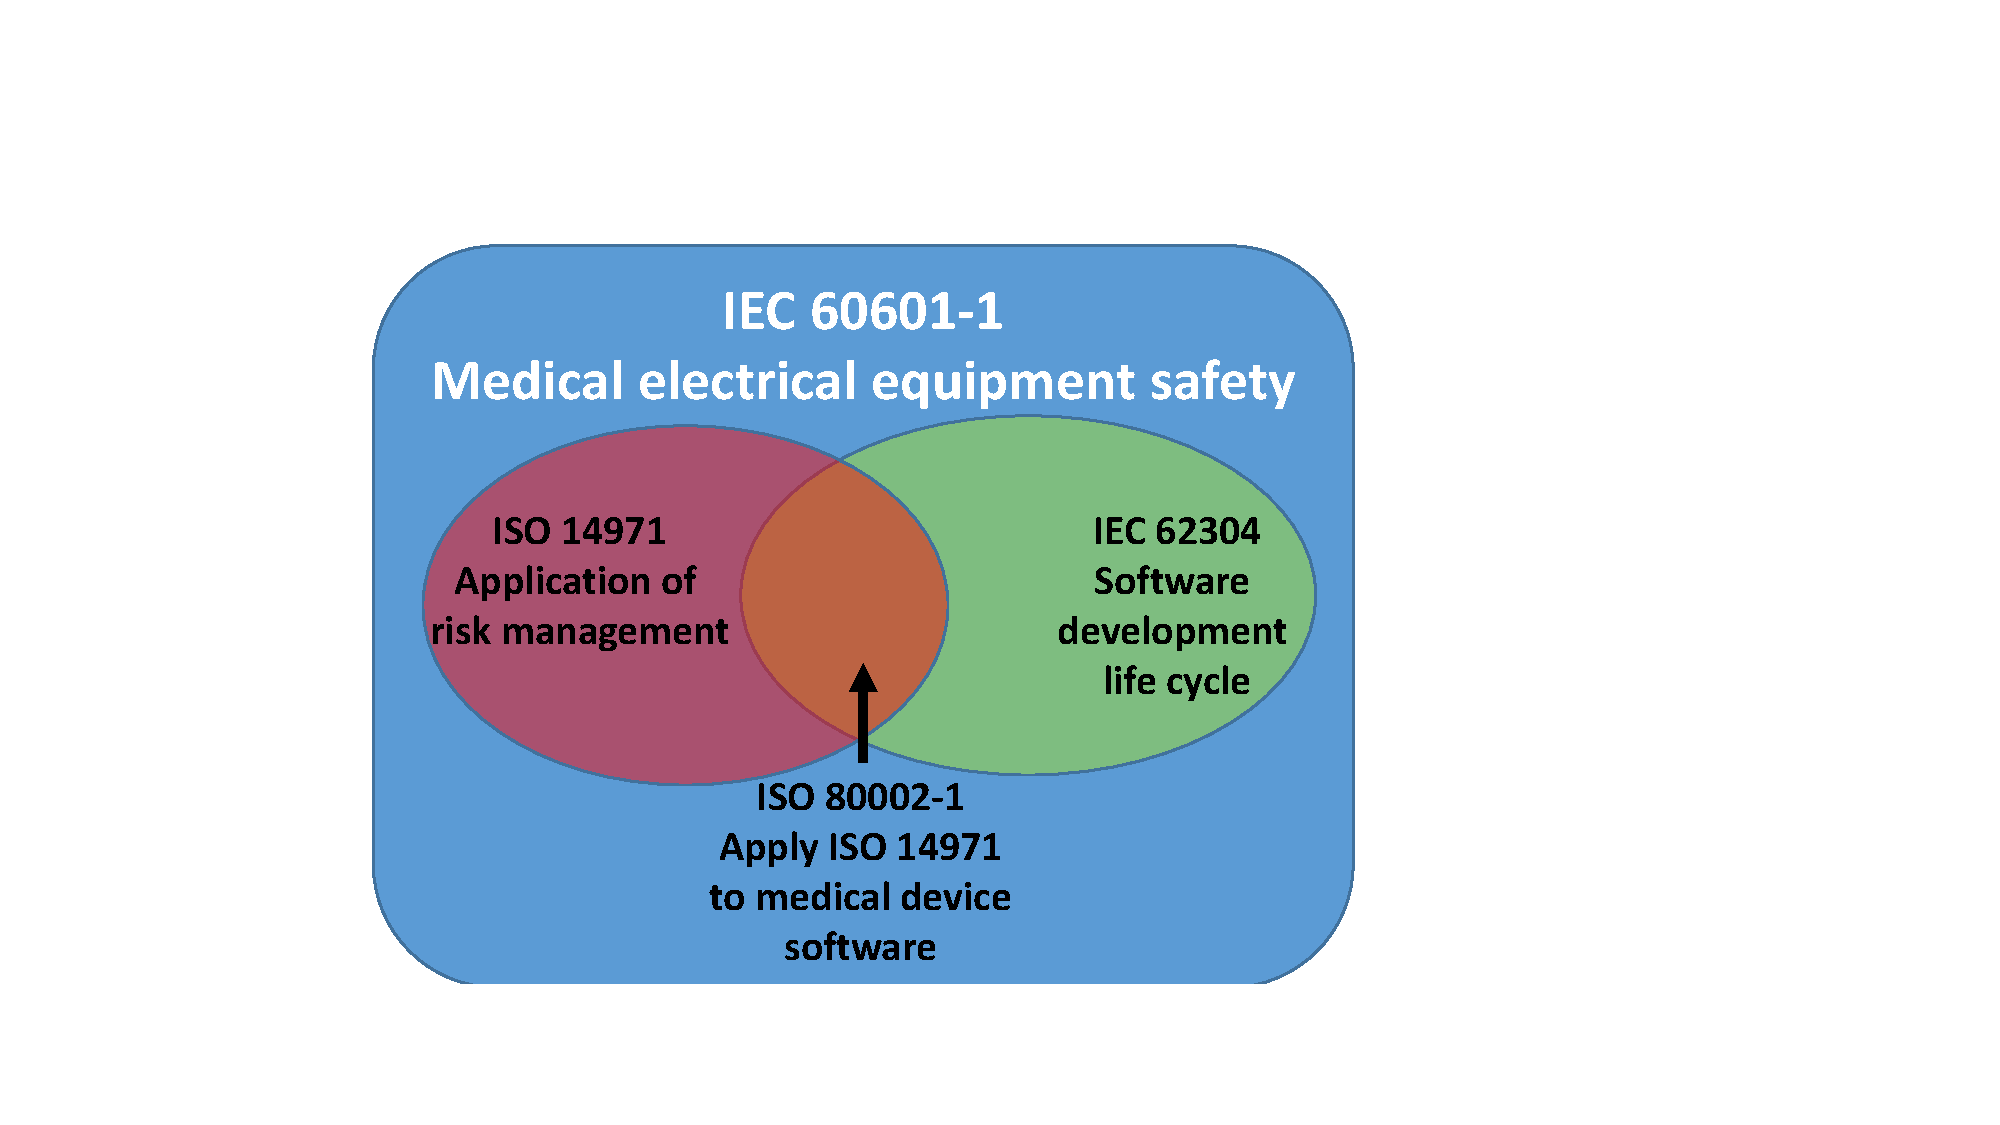
\includegraphics[width=0.6\textwidth]{figs/stardards.pdf}
		\caption{\small International standards for medical device safety. These standards define the required activities during the development process.}
		\label{fig:standards}
\end{figure}

%\subsection{Safety Standards During Development}
\figref{standards} describes the primary standards to enforce medical device safety and their relationships. 
The basic rationale behind these standards is that: if all the risks/hazards of the device are identified and reasonably mitigated, and the device is developed with rigorous process, the device is \emph{reasonably safe}. 
The IEC 60601 Medical Electrical Equipment - General requirements for basic safety and essential performance is a product safety standard that all electronic medical devices must comply to. 
IEC 60324 specifies the processes and activities needed to perform during the software development life cycle to ensure software safety. 

Risk management is a core activity throughout the software development life cycle.
 ISO 14971 is specified for the application of risk management to medical devices. 
In addition, for each risk management activity of ISO 14971, ISO 80002-1 provides additional guidelines for the software component, which highlights and explains approaches to assuring that software safety is adequately addressed.
%%On similar lines, in the European Union there are five medical devices categories based on non-invasive vs. invasive, length of stay in body, contact with blood vessels or the central nervous system, active vs. non-active and implantable devices. (\cite{EU_classify}) 
%%Invasive devices with active interventions are subject to stringent regulations to ensure the patient's safety and efficacy of therapy.
%\begin{figure}[t]
		%\centering
		%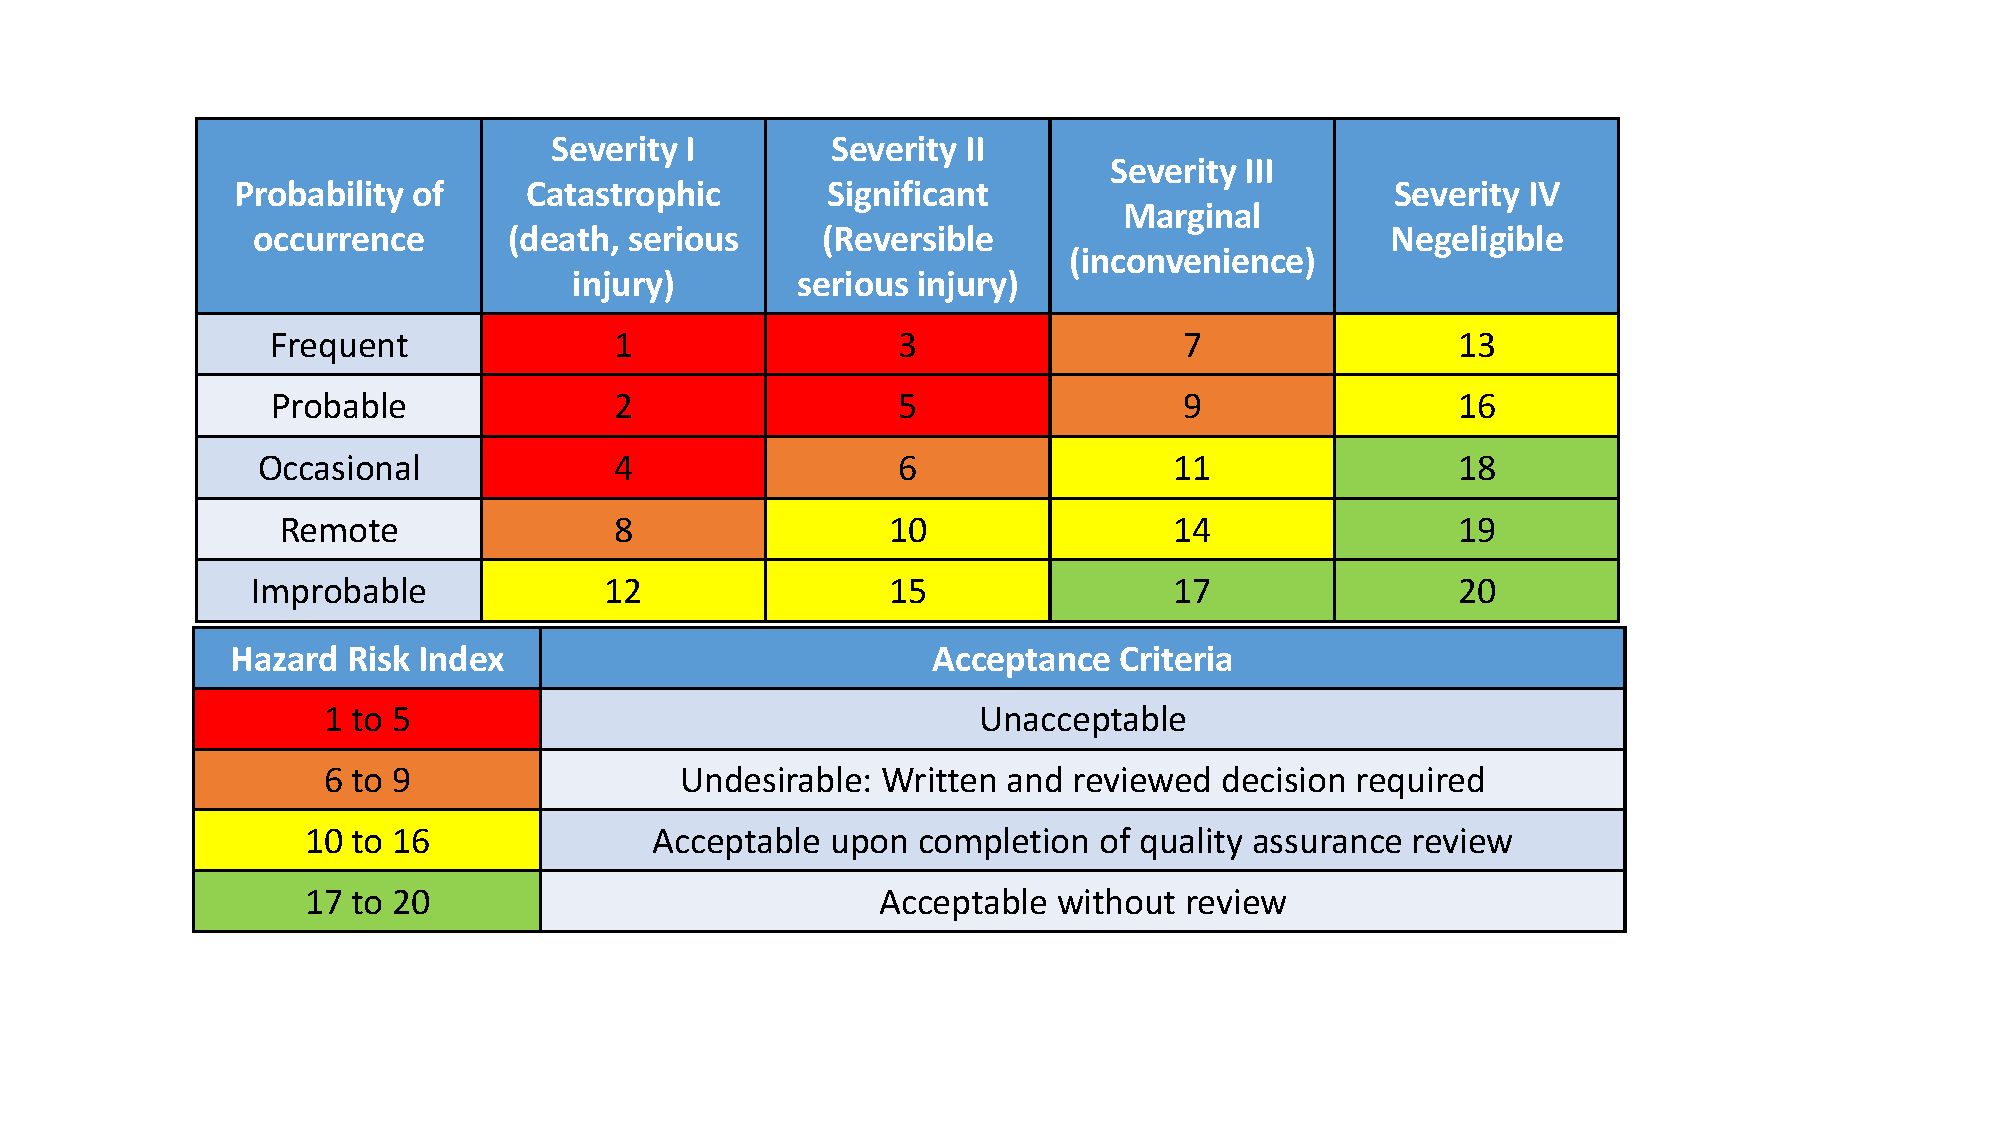
\includegraphics[width=\textwidth]{figs/risk_analysis.pdf}
		%\caption{Top table: Risk index according to occurrence and severity. Bottom table: Risk control using risk index}
		%\label{fig:risk_ana}
%\end{figure}



\subsection{Pre-Market Evaluation with Clinical Trials}
%Regardless of how rigorous the risk management and the device development process are, the devices have to be able to achieve their design goal on the real patient, which can only be evaluated within its physiological environment. 
Devices that have high risk factors are required to submit clinical evidence for their safety and efficacy, often in form of clinical trials. 
In clinical trials, the devices are used on a preselected population of patients following carefully-designed protocols. 
The goal of a medical trial, in part, is to obtain unambiguous results for the primary question of the trial which can support the safety and/or efficacy of the devices. 
However, conducting clinical trials is very time consuming and expensive, and risks found during clinical trials are very expensive to fix (\cite{trialcost}). 

%To address this \textbf{safety gap} between ensuring the device satisfies its therapeutic requirements with the patient-in-the-loop and testing its software specifications, new approaches for closed-loop validation of the device software within the physiological context are needed - this is the primary focus of this article.




%\section{Current Testing, Validation and Verification Approaches}
%In order to facilitate the early detection and correction of any software defects, the FDA has focused on infusion pumps due to the large number of recalls. In April 2010, the FDA began the ``Infusion Pump Improvement Initiative" which offers manufacturers ``the option of submitting the software code used in their infusion pumps for analysis by agency experts prior to premarket review of new or modified devices." 	\cite{}
%
%An effective software verification methodology is therefore needed for the risk analysis and certification of medical device software during the pre-market submission phase. While formal methods of verification are used for medical device software (\cite{challenge, challenge2, challenge3}), testing continues to be required because it can expose different kinds of problems (e.g. compiler bugs), can examine the program in its system context, and increases the diversity of evidence available. Testing for medical device software currently is ad hoc, error prone, and very expensive. Traditional methods of testing do not suffice as the test generation cannot be done independently of the current state of the patient and organ. The primary approach for system-level testing of medical devices is unit testing using a playback of pre-recorded electrogram and electrocardiogram signals (\cite{testing_imd, Vip}). This tests if the input signal triggers a particular response by the pacemaker, but has no means to evaluate if the response was appropriate for the patient condition. Furthermore, this approach of ``tape testing''\Hao{elaborate} is unable to check for safety violations due to inappropriate stimulus by the pacemaker. Pacemaker Mediated Tachycardia (PMT), a condition that is described later in this paper, is a strong example of why we need a model of the heart such as the one presented in this paper, which can be used for closed-loop system analysis. 
%PMT is a condition where the pacemaker inappropriately drives the heart-rate toward the upper rate limit. With a tape test, PMT would not occur and the response of the pacemaker could be classified as appropriate therapy.
%\begin{figure}[t]
		%\centering
		%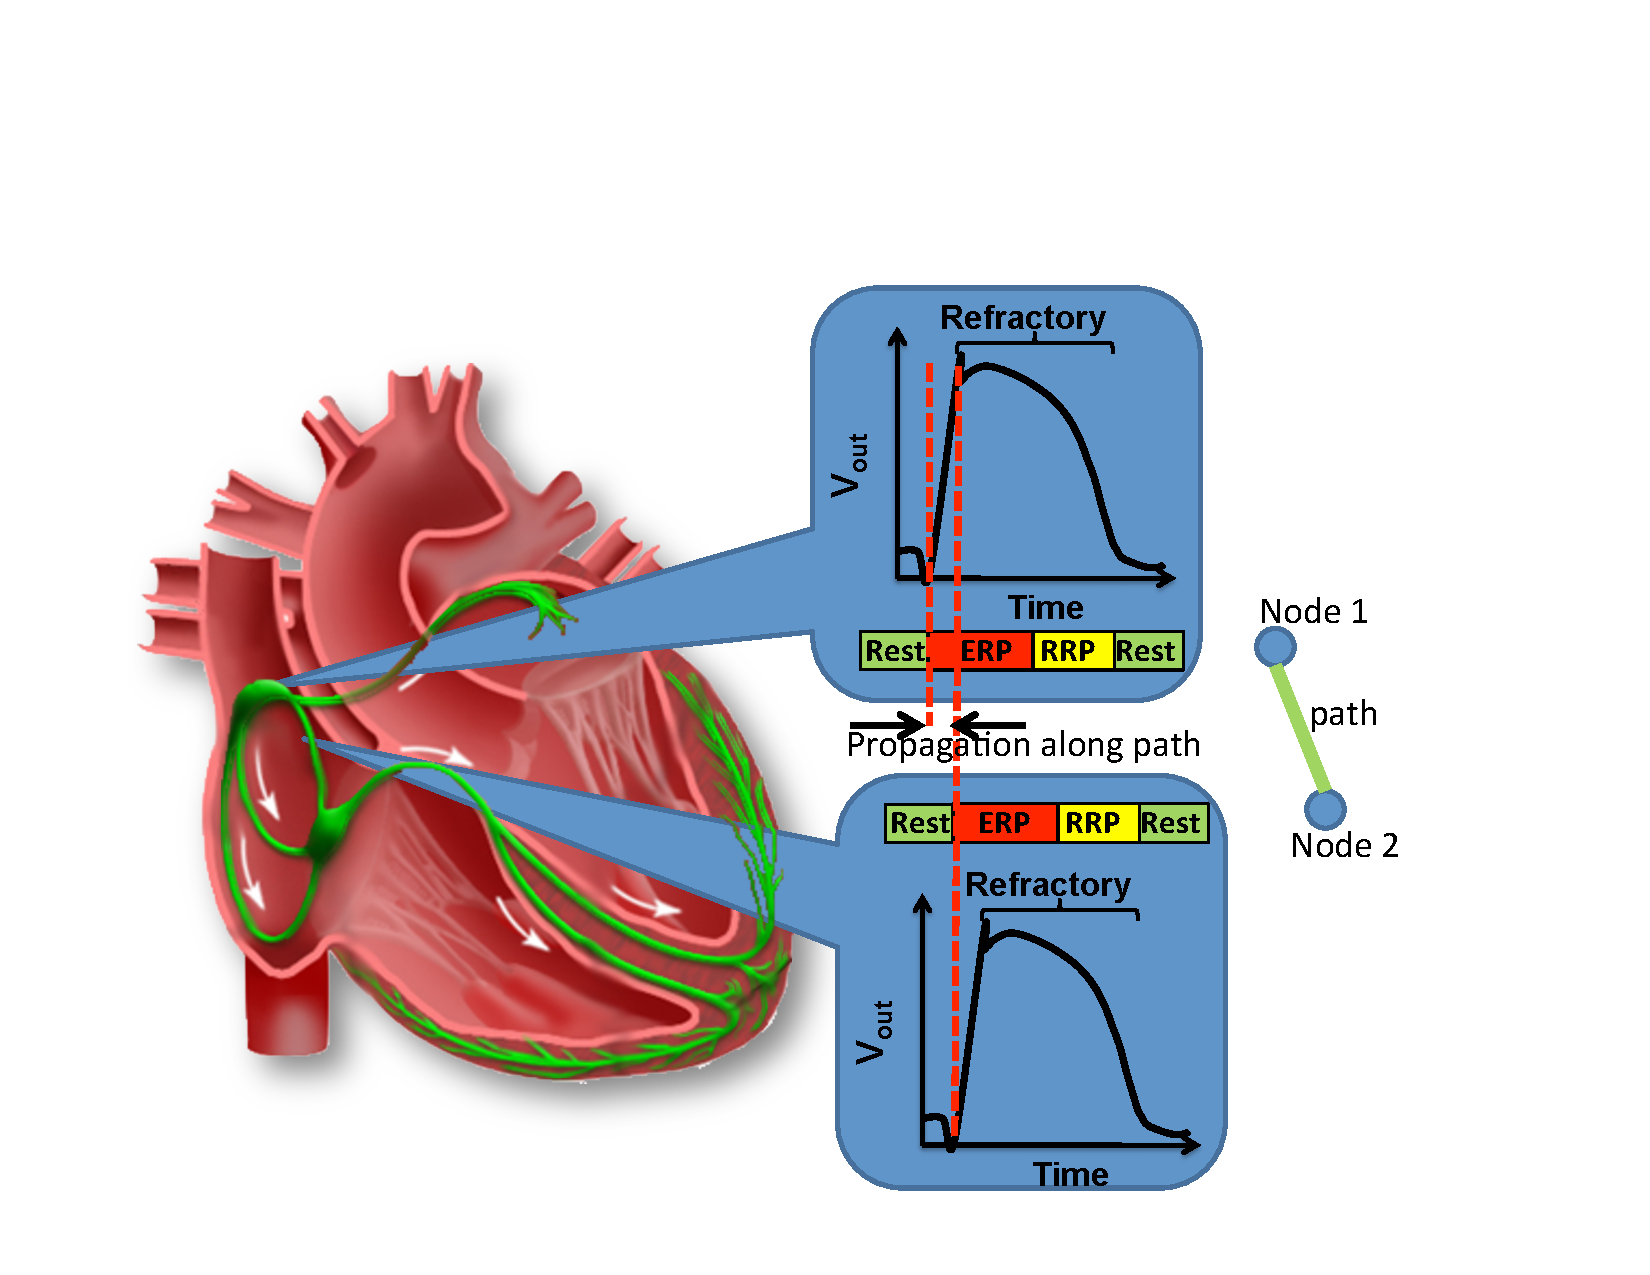
\includegraphics[width=0.8\textwidth]{figs/heartmodel.pdf}
		%%\vspace{-5pt}
		%\caption{\small By extracting timing and electric conduction information we model the signal activation, refractoriness and propagation across the heart tissue as a set of node and path automata.}
		  %%\vspace{-15pt}
		%\label{fig:heartmodel}
%\end{figure}
%As the testing environment (i.e., patient condition) is not entirely under the control of the tester, the problem changes significantly as a degree of nondeterminism is introduced in the process. Implantable medical devices are a primary example of Medical Cyber-Physical Systems where the safety and efficacy of the device and device software must be evaluated within a closed-loop context of the patient. The key challenge is in the generation of physiologically relevant tests such that the device does not provide inappropriate therapy, and does not adversely affect the safety of the patient. In addition, test generation must be interactive and adaptive such that the previous test stimulus affects the current state of the patient. The test generator must consider the current state when generating the next input in a way that advances the purpose of the test. The problem becomes one of the controller synthesis problems and cannot be addressed by an off-the-shelf model checker~\cite{rushby}.  
   %
%Formal methods have traditionally been used for verification of time-critical and safety-critical embedded systems \cite{form-meth}. Until recently, these methods have not been used for medical device certification. \cite{med-form3} presented the use of Extended Finite State Machines for model checking of a resuscitation device. Formal techniques have also been applied to improve medical device protocols (\cite{med-form2}) and safety (\cite{med-form1}), but the authors either used a simplified patient model or did not model the patient at all. 
\subsection{Lack of Closed-loop Validation During and After Device Development}
While formal methods are used for medical device software validation (\cite{challenge, challenge2, challenge3}), testing continues to be the primary method for safety and efficacy evaluation during device development.
Testing for medical device software currently is ad hoc, error prone, and very expensive. 
Traditional methods of testing do not suffice as the test generation cannot be done independently of the current state of the patient and organ. 
The primary approach for system-level testing of medical devices is unit testing using a playback of pre-recorded electrogram and electrocardiogram signals (\cite{testing_imd, Vip}). 
This tests if the input signal triggers a particular response by the device, but is unable to check how the device affects the physiological conditions of the patient.

The only closed-loop validation activity is clinical trials, which is very expensive and expose the patients to uncertified devices. 
Issues found during clinical trials are also expensive to fix.
There is urgent need for closed-loop validation approaches during and after device development to provide safety and efficacy confidence to the device design.
\section{Model-based Design and Pre-certification of Medical Devices}
%With the deluge of software-based closed-loop medical devices in the coming years, relying on clinical trials as the only closed-loop evaluation method to identify risks rooted in device software is not scalable. 
In industries like automotive and avionics, mathematical models of the physical environment that the system operates in are developed for analyzing the safety and efficacy of the control systems (or their models) (\cite{autosar, avsi}).
Similar approaches can potentially help during the development process of autonomous medical devices and provide extra confidence to the devices before conducting clinical trials. 
However, unlike man-made systems like automobiles and aircrafts, physiological systems are less understood with larger variations for the type and degree of patient conditions. 
The lack of faithful models of physiological environment for the autonomous medical devices is one of the reason that model-based approaches are not well-adopted in the medical device industry. 
\begin{figure}[t]
		\centering
		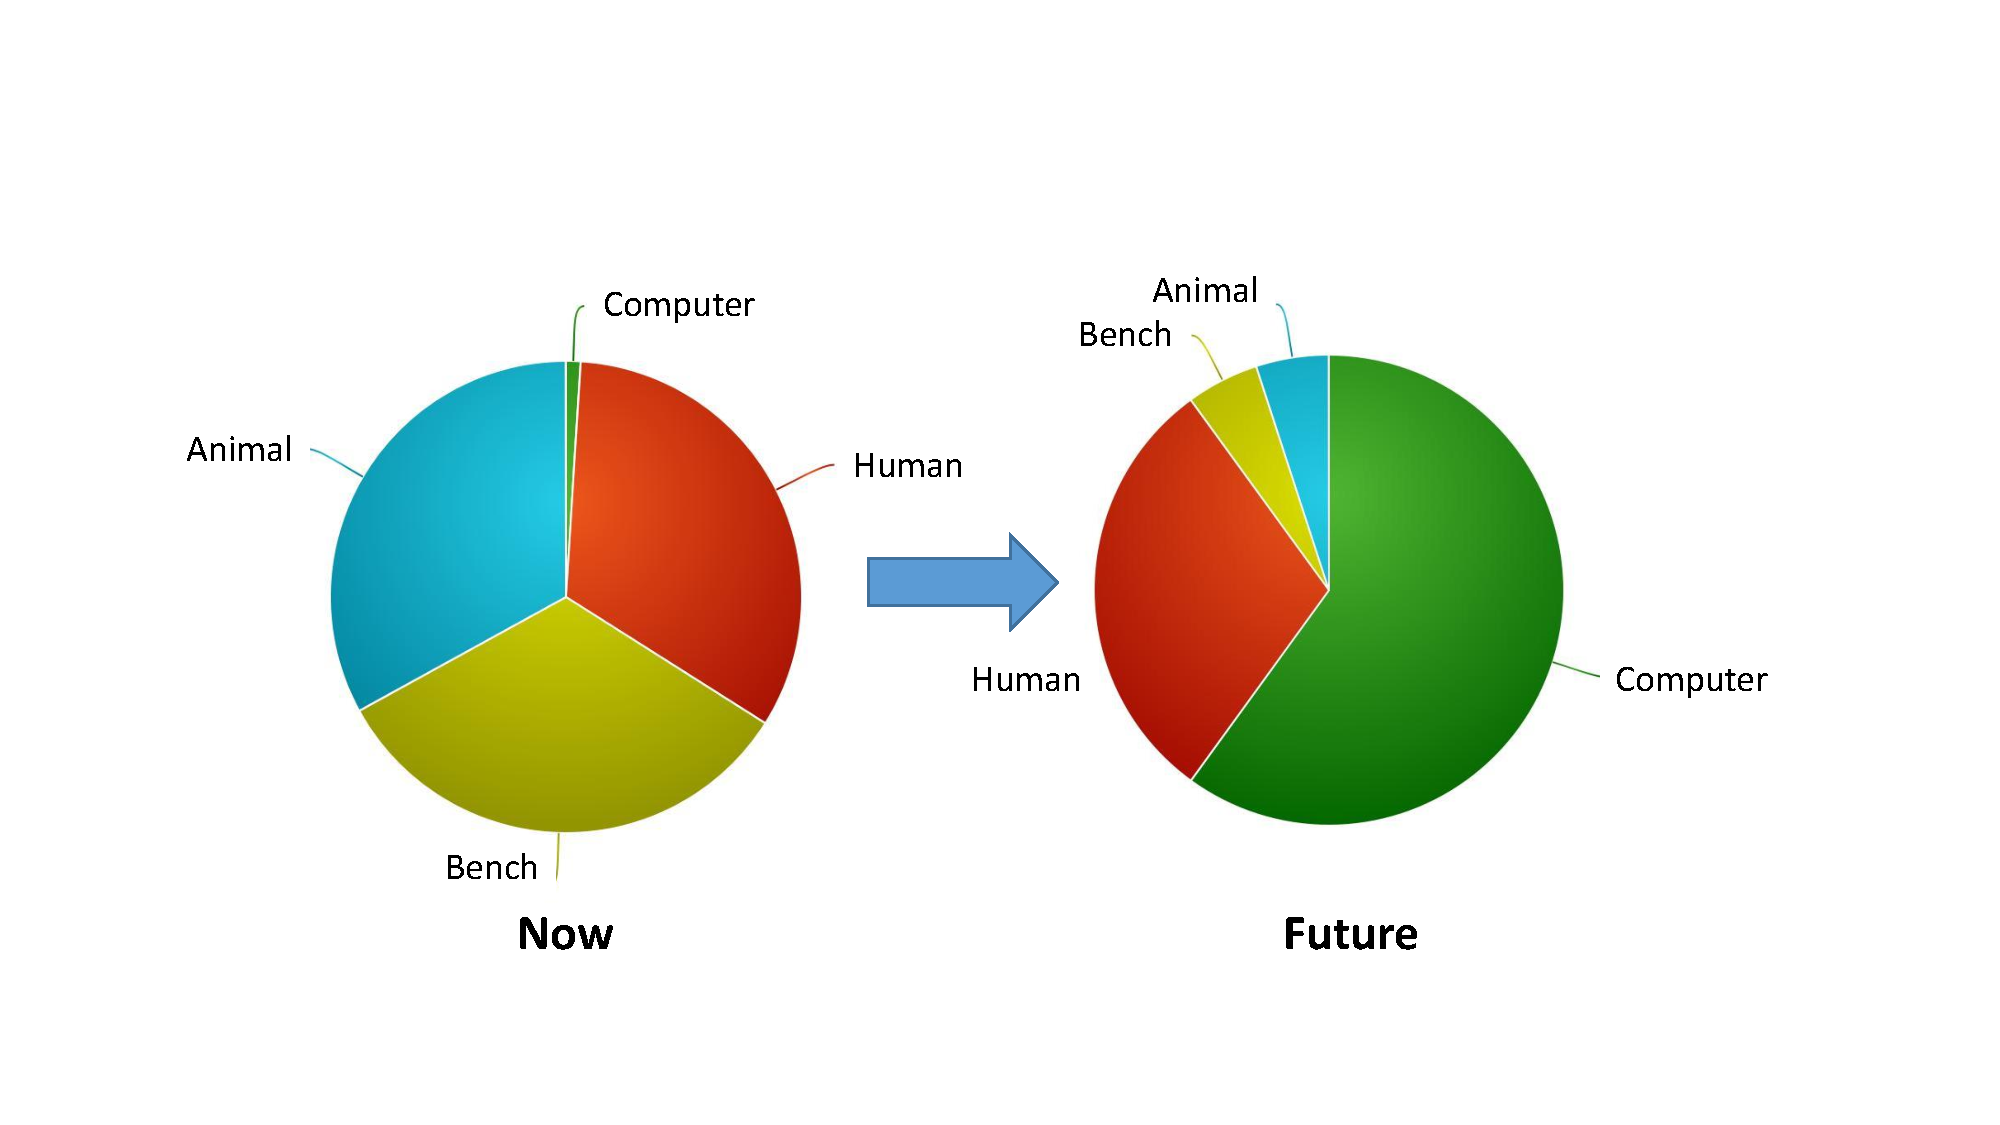
\includegraphics[width=\textwidth]{figs/MDIC.pdf}
		\caption{\small Percentage of computer simulation is expected to increase as safety and effectiveness evidence of medical devices (http://mdic.org/)}
		\label{fig:MDIC}
\end{figure}

As computational models of human physiology are developed, they can be used to interact with closed-loop medical devices or their models. 
The FDA is starting to recognize in-silico modeling and simulation as regulatory-grade evidence for device safety and efficacy. 
For example, \cite{pancreas_paul} developed glucose-insulin models that can be used to evaluate control algorithms for artificial pancreas devices which can sense blood glucose and deliver insulin. 
Simulation results with the models have been recognized by FDA to replace animal trials, in part, which significantly reduced cost (\cite{pancreas}). 
With the increasing interest and recognition from the regulators, computer models and simulations are expected to play bigger role as as ``regulatory-grade evidence" evidence in the development of future closed-loop medical devices (\figref{MDIC}).

\section{Contributions}
In this dissertation, implantable cardiac devices are used as working examples to demonstrate how model-based approaches can help improve the safety and efficacy of autonomous medical devices during and after their development. 
By demonstrating the process of developing verified models to generate verified code of the devices, the results of model-based closed-loop validation can provide confidence towards the safety and efficacy of the devices.

The contribution of this dissertation is fourfold:
\begin{enumerate}
	\item \textbf{Clinical Electrophysiology heart model structure: }A heart model structure was developed that can represent a large variety of heart conditions and interact with implantable cardiac devices in closed-loop. The heart model structure is available in both software and hardware for different applications of closed-loop validation.
	\item \textbf{Automated heart model abstraction and refinement: }An abstraction tree structure was developed to abstract the heart models to capture the large variability of heart conditions during closed-loop model checking of implantable pacemaker, and refine the heart models to provide physiological interpretability to the counter-examples.
	\item \textbf{Automated model translation for code generation: }An automated model translation tool UPP2SF was developed to translate verified UPPAAL device model to Stateflow model, which allows rigorous translation from model to C code.
	\item \textbf{in-silico Pre-clinical trials: }A large virtual population of heart models was generated to evaluate the VT/SVT discrimination algorithms of Implantable Cardioverter Defibrillators before clinical trials.
\end{enumerate}

\begin{figure}[t]
		\centering
		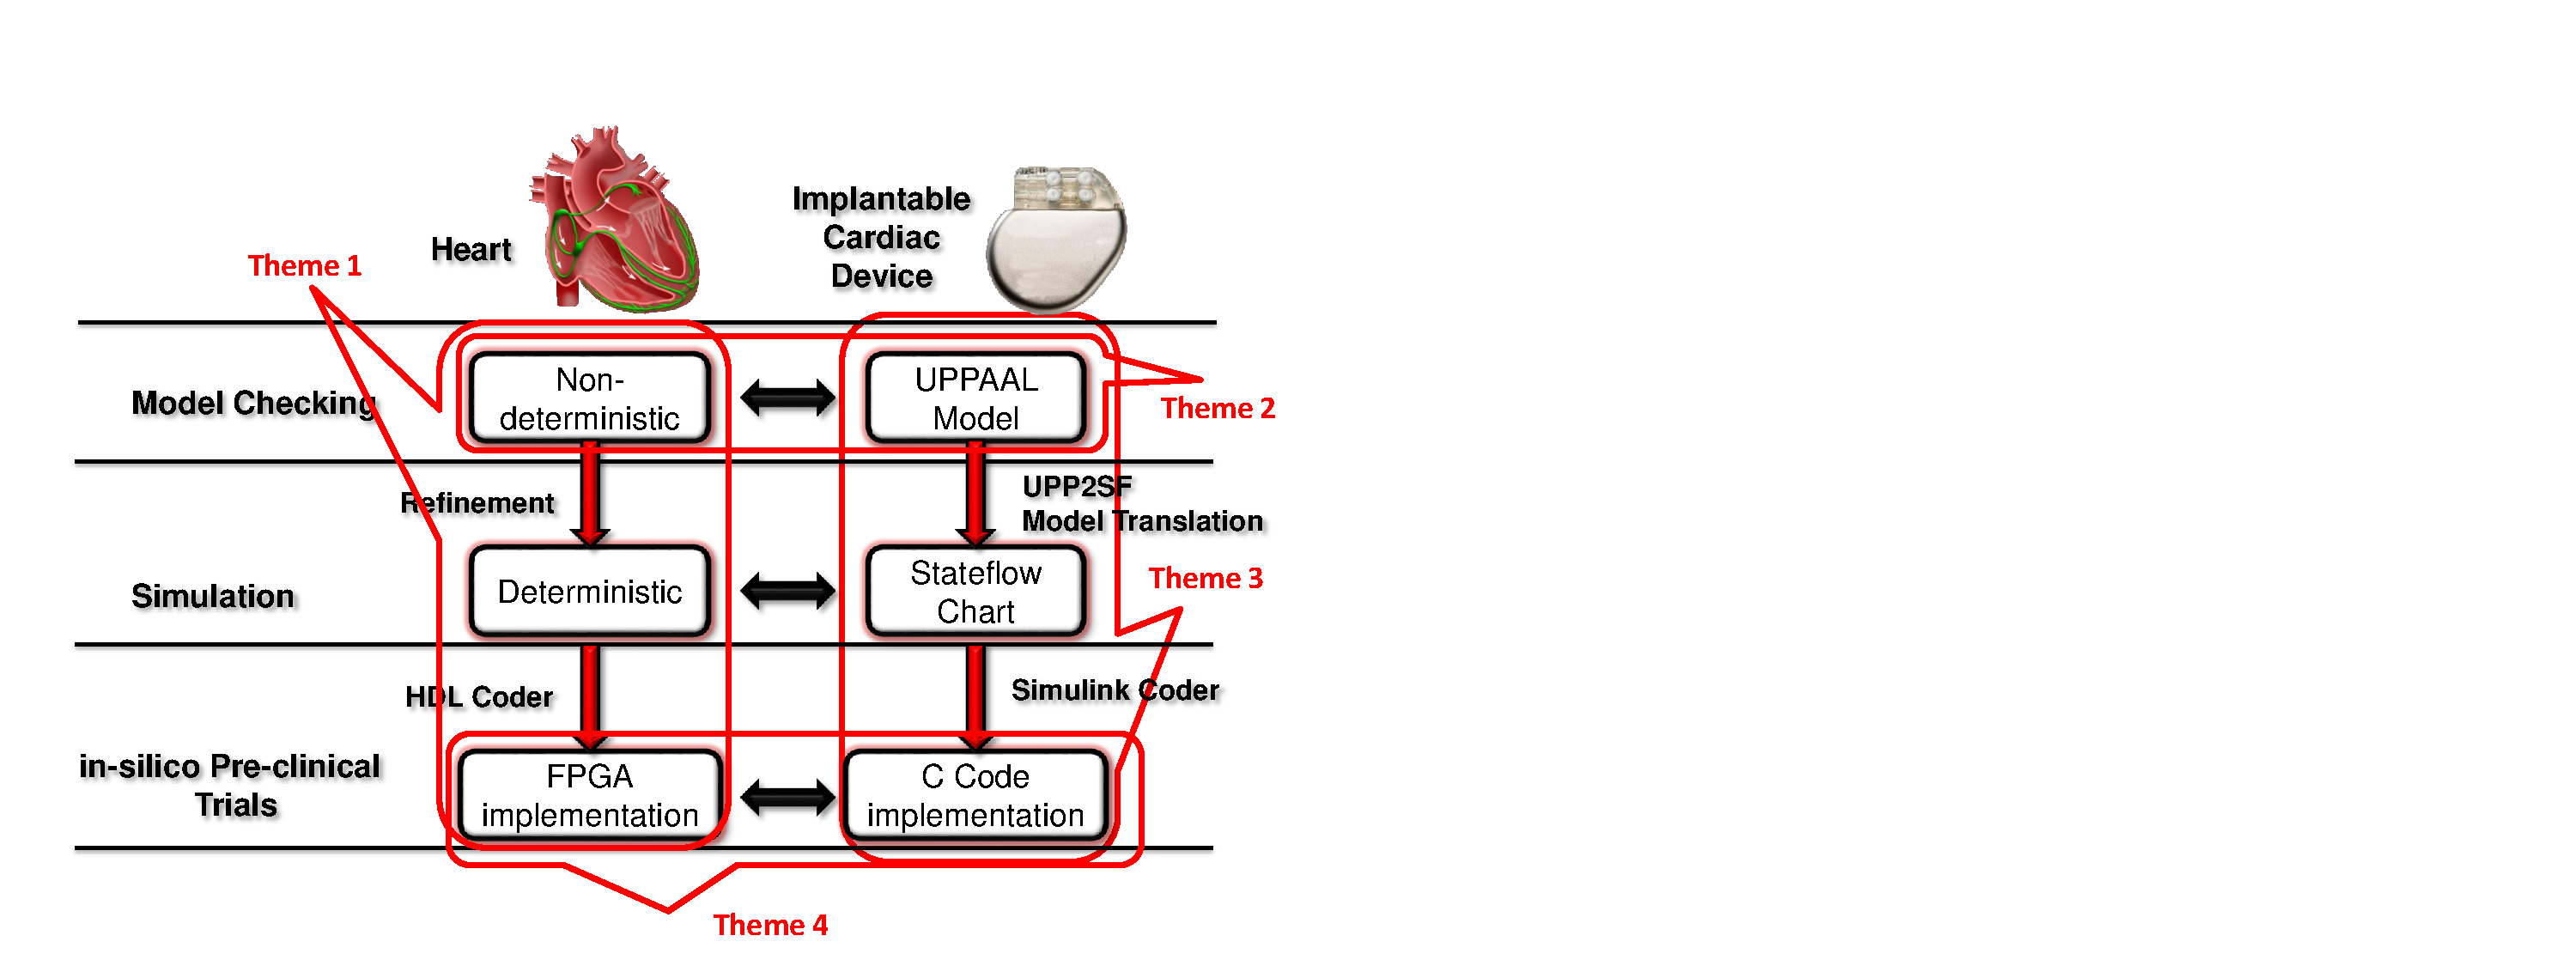
\includegraphics[width=0.8\textwidth]{figs/model_based_b.pdf}
		%\vspace{-5pt}
		\caption{\small Model-based design for implantable cardiac devices with closed-loop validation}
		  %\vspace{-15pt}
		\label{fig:modeling_overview}
\end{figure}

Fig. \ref{fig:modeling_overview} demonstrates the structure of the dissertation.
The dissertation can be broken down into 4 themes, which are illustrated in \figref{modeling_overview}. 

The remaining dissertation is arranged as follow:
Chapter 2 discusses a dual chamber pacemaker design (\cite{compass}) as the motivating example to illustrate the safety hazards that the device may pose to the patients.
Chapter 3 discusses the physiological models that are necessary for closed-loop evaluation of medical devices, and how to use those models to represent complex physiology with large variability \cite{VHM_proc}.
Chapter 4 discusses the use of model-checking techniques to evaluate the safety and efficacy of device design early in the device design stage, with focus on the abstraction and refinement of the heart models to cover large variety of physiological conditions (\cite{STTT13}).
Chapter 5 discusses the rigorous translation from verified device model to device implementation which maintains the verified properties (\cite{RTAS12}).
Chapter 6 discusses the in-silico pre-clinical trial, which the devices are evaluated on a virtual patient cohort consists of physiological models to provide useful insights for planning a clinical trial. 

%The contribution of this effort is three-fold: (a) We developed an integrated functional (i.e., clinically-relevant) and formal (i.e., timed automata based) Virtual Heart Model  (VHM) (see \figref{heartmodel}) and a pacemaker device model for interactive and clinically relevant test generation.  (b) We provide a set of general and patient condition-specific pacemaker software requirements to ensure the safety of the patient is met under all cases, and (c) We provide a means to test and verify the closed-loop system over a variety of basic operation tests where the heart rate must be maintained, the atrial-ventricle synchrony must be enforced and complex closed-loop tests, where the pacemaker must not initiate tachycardia or perform improperly during lead displacement. With this approach of model-based testing, an executable functional model of the pacemaker is created at an early stage in the development process. This model-based methodology is an early step in addressing the urgent need for pre-market evaluation of medical device design and certification.

\section{Useful terminologies for often misinterpreted terms}
Ensuring the safety and efficacy of complex medical devices has drawn interest not only from stakeholders like regulators and industries, but also medical professionals and academia. 
Different communities have different interpretations over certain terminologies, often causing misunderstandings. 
In this dissertation, terminologies from the regulation perspective are adopted. 
Most of the definitions are referred from the FDA guideline document General Principles of Software Validation (\cite{fda2}). 
Below are several terminologies that are used throughout the dissertation which worth clarifying.
\subsection{Requirements vs. Specifications}
By the definition of the FDA (\cite{fda3}), the requirements of a system describe \textbf{what} the system should achieve and the specifications of a system describe \textbf{how} the system is designed to satisfy the requirements. 
For instance, a requirement for an autonomous car is "The car should not hit objects". 
The corresponding specification can be "brake if the speed of the car is greater than $x$ and the distance to the object is less than $y$". 
It is obvious that a car satisfying its specification may not satisfy the requirement (e.g. when the car is driving too fast or the obstacle pops up right in front of the car). 
In this dissertation, the word requirement in particular denotes the intended uses of the medical devices to improve physiological conditions.

\subsection{Validation vs. Verification vs. Testing}
As defined in \cite{fda2}, software validation is the confirmation by examination and provision of objective evidence that:
\begin{enumerate}
	\item software specifications conform to user needs and intended uses, and 
	\item the particular requirements implemented through software can be consistently fulfilled
\end{enumerate}
The first aspect ensures the device is safe and effective. 
The second aspect maintains the traceability of requirements throughout the development life cycle.
Software verification fulfills the second aspect of software validation by "providing objective evidence that the design outputs of a particular phase of the software development life cycle meet all of the specified requirements for that phase. "
\begin{figure}[t]
		\centering
		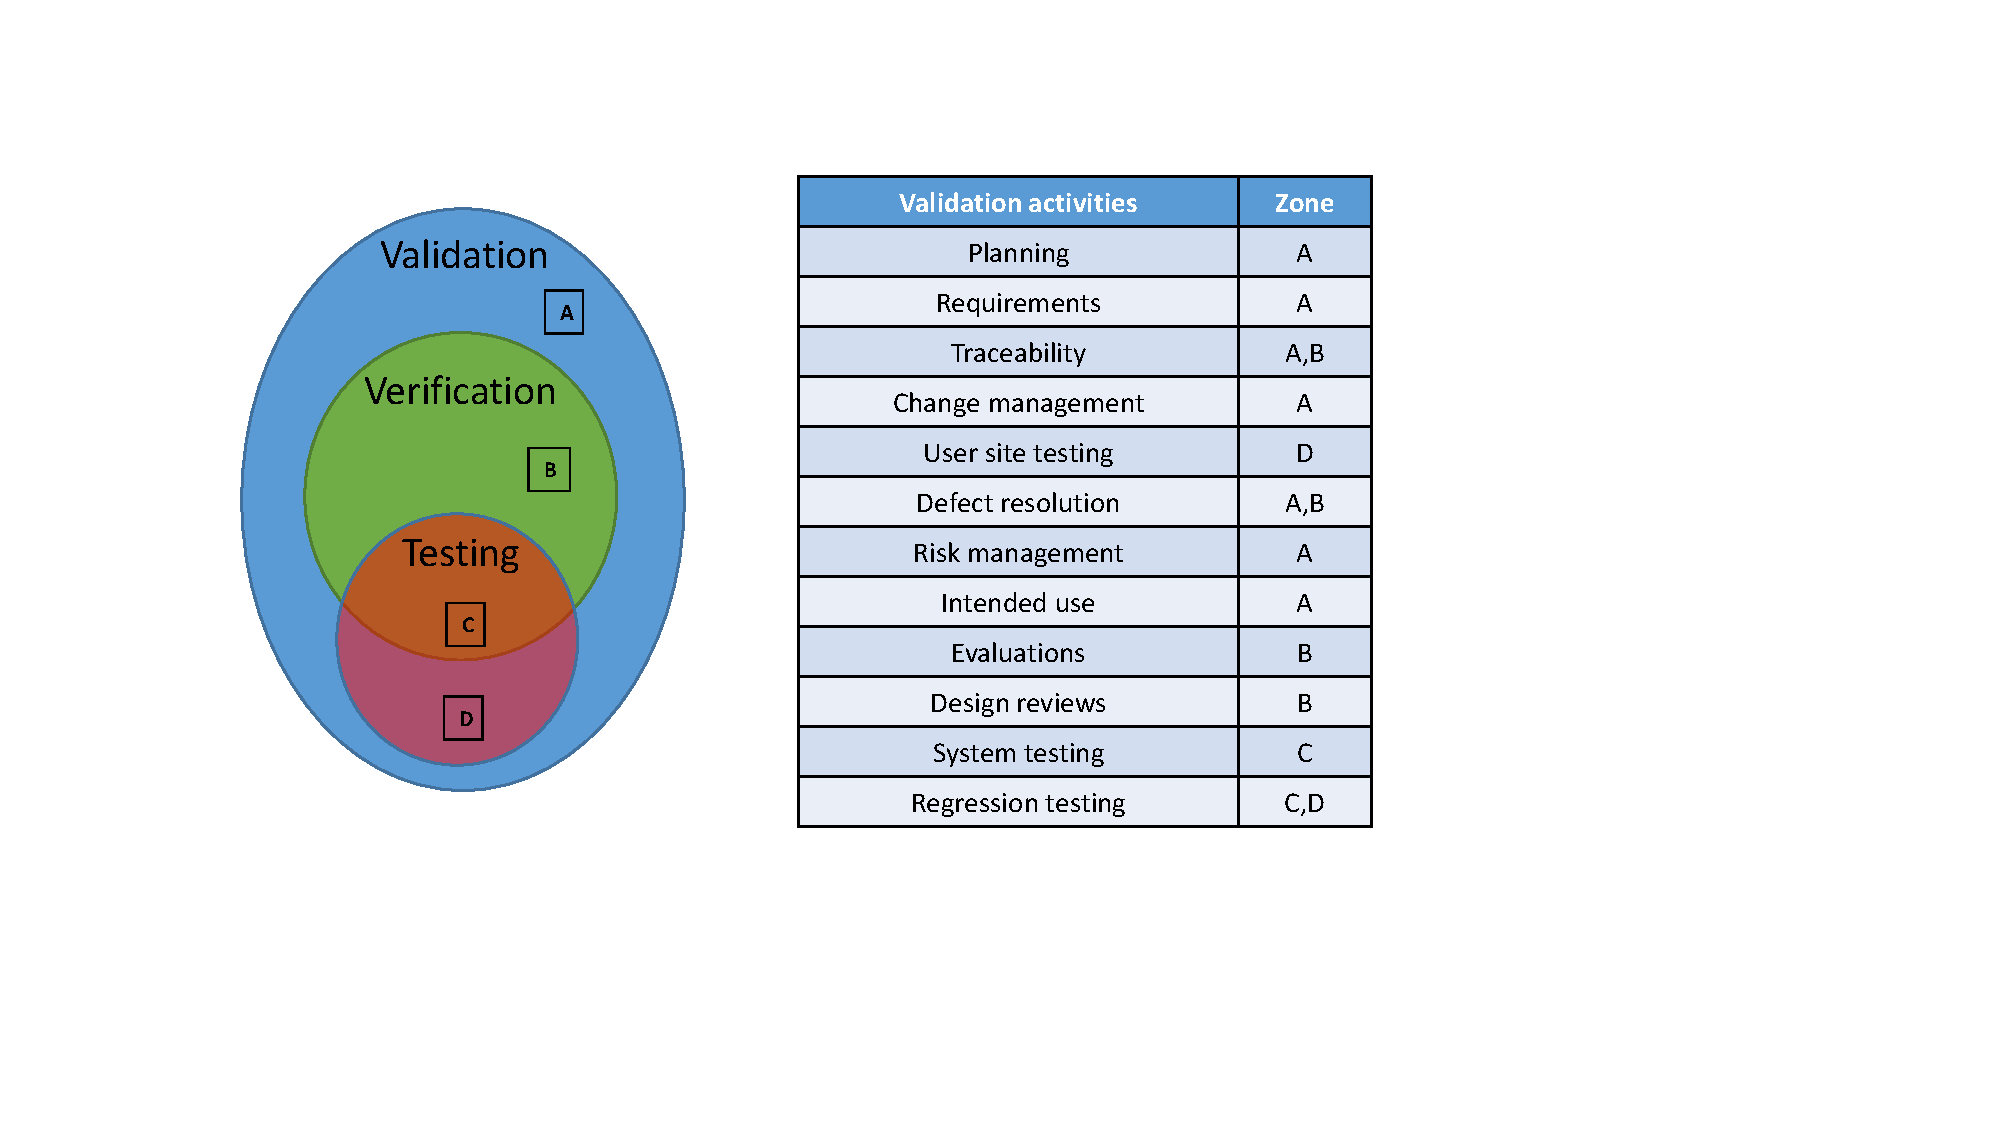
\includegraphics[width=\textwidth]{figs/validation.pdf}
		\caption{Validation activities during the software development life cycle (\cite{Vogel})}
		\label{fig:validation}
\end{figure}

Testing is the technique that can be used for validation and/or verification. \figref{validation} illustrates the relationship between validation, verification and testing, and different activities during the software development life cycle to ensure the safety and effectiveness of the software.
\subsection{Closed-loop vs. Open-loop Evaluation}
In open-loop evaluation, i.e. open-loop testing, input sequences are send to the system and system outputs are compared with expected outputs. 
In open-loop testing, the system outputs do not affect the inputs afterward. 
In closed-loop evaluation, the environment of the system is taken into account. 
System outputs affect the state of the environment and thus affect the input sequences. 
For closed-loop medical devices, clinical trials are currently the most common closed-loop evaluation method. 
Enabling closed-loop evaluation during device design requires models of the environment, which is human physiology for closed-loop medical devices.

Closed-loop evaluation accomplishes two goals in model-based design: 1) It enforces environmental constraints so that the test space is smaller and the test cases have physiological relevance, 2) Execution traces can be better interpreted as the physiological models encode domain knowledge. 
%%Through each of the chapters to follow, we cover different aspects of modeling the physiological system and the device, validating the models, running model checking on the closed-loop system and testing the deterministic systems derived from the abstract models. With the goal of 

%%The US Food and Drug Administration defines medical device an instrument, apparatus, implement, machine, contrivance, implant, in vitro reagent, or other similar or related article, including a component part, or accessory which is:
%%\begin{itemize}
%%	\item recognized in the official National Formulary, or the United States Pharmacopoeia, or any supplement to them
%%	\item intended for use in the diagnosis of disease or other conditions, or in the cure, mitigation, treatment, or prevention of disease, in man or other animals, or
%%	\item intended to affect the structure or any function of the body of man or other animals, and which does not achieve any of its primary intended purposes through chemical action within or on the body of man or other animals and which is not dependent upon being metabolized for the achievement of any of its primary intended purposes."
%%\end{itemize}
\chapter{A Motivating Example: A Dual Chamber Pacemaker Design}
Intuitively, an autonomous medical device like pacemaker should satisfy the following requirements: 1) improve unhealthy physiological conditions of a patient (efficacy), and 2) not to deteriorate current physiological condition (safety).
Evaluating both requirements requires understanding of the physiological environment the device is in.
In the following sections, the physiological basis for the heart and the pacemaker is introduced, followed by a dual chamber pacemaker specification (\cite{compass}).
Potential safety hazards for a pacemaker were then analyzed and two known safety hazards were discussed in detail.
The dual chamber pacemaker specification is then used throughout the thesis to demonstrate how different model-based techniques can be used to validate the safety and efficacy of an autonomous medical device.
\section{Physiology Basis of the Heart and the Pacemaker}
First, we use this small section to introduce the physiology basis of the heart and the application of implantable cardiac devices. 
Readers with knowledge of this subject can skip to the following sections.
\subsection{Blood Circulation System}
The heart is the "motor" for blood circulation within our body. The heart has two ventricles which pump the blood out of the heart, and two atria which gather blood from the body and pump them into the ventricles. (\figref{circulation}.(a)) There are two circulations through the heart: the \emph{Pulmonary circulation} and the \emph{Stemic circulation}. In the pulmonary circulation, the right atrium collects oxygen-depleted blood from all over the body and pumps it into the right ventricle. The right ventricle then pumps low-oxygen blood to the lungs. The blood gets oxygenated in the lungs and gathers into the left ventricle. In the stemic circulation, the oxygenated blood in the left atrium is pumped into the left ventricle. The left ventricle pumps the blood to the rest of the body and the heart itself. After the body extracts the oxygen from the blood and injects carbon dioxide, the oxygen-depleted blood then flows back to the right atrium.
\begin{figure}[!t]
\centering
		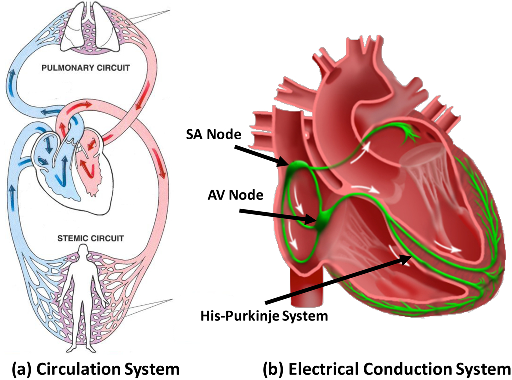
\includegraphics[width=0.9\textwidth]{figs/circulation.pdf}
		
%\vspace{-10pt}
\caption{\small (a) The circulation system (\cite{circ}). (b) Electrical Conduction system of the heart}
\label{fig:circulation}
%\vspace{-15pt}
\end{figure} 
\subsection{Electrical Conduction System of the Heart}
The oxygen demand of the body changes during different activities. For example, the demand is higher while running and lower while sleeping. To satisfy these demands, the heart muscles in the atria and the ventricles have to contract with certain pattern and frequency in accordance to optimize the \emph{Cardiac Output}, which refers to the volume of blood pumped by the heart per minute (mL blood/min). The coordinated contractions of the heart muscles are governed by the electrical conduction system of the heart (\figref{circulation}.(b)) A \emph{Normal Sinus Rhythm (NSR)} is the healthy heart rhythm which provides efficient blood flow. During a NSR, electrical signals are periodically generated by the \emph{Sinoatrial (SA) node} in the upper right atrium, which acts as the intrinsic pacemaker of the heart. The signals conduct throughout both atria and trigger muscle contractions to push blood into the ventricles. After a long conduction delay at the \emph{AV node} so that both ventricles are fully filled, the signals conduct through fast-conducting \emph{His-Purkinje} system to trigger almost simultaneous contractions of the ventricles and pump blood out of the ventricles. 

Derangement from NSR can result in insufficient cardiac output and thus insufficient oxygen supply to the body and/or the heart itself, which are referred to as \emph{Arrythmia}. Arrhythmia impair the heart's ability to efficiently pump blood and compromise the patient's health. 
Arrhythmia are categorized into so-called \emph{Tachycardia} and \emph{Bradycardia}. Tachycardia features undesirable fast heart rate which can cause inefficient blood pumping. Bradycardia features slow heart rate which results in insufficient blood supply. Bradycardia are due to failure of impulse generation with anomalies in the SA node, or failure of impulse propagation where the conduction from atria to the ventricles is delayed or blocked. 
\subsection{Electrophysiology and Implantable Cardiac Devices}
\label{EP}
The electrical activities of the heart closely couple with the mechanical contractions thus the electrical activities of the heart can be monitored and used to diagnose arrhythmia. The most well-known method is Electrocardiogram (ECG), which measures the integration of electrical activities of the heart measured along different axis on the body surface. The electrical activities can also be directly measured by inserting electrodes through the vein into the heart. The electrodes are placed against the inside heart wall and localized electrical activities can be measured. Physicians can also deliver pacing sequence through the electrodes to explore the heart conditions. This procedure is referred to as Electrophysiological (EP) Testing  (\cite{josephson}) and the signals are referred to as electrograms (EGMs) (\figref{probes}.b). The timing and morphology of the  ECG and EGM signals together are used to diagnose arrhythmia.
\begin{figure}[!t]
\centering
		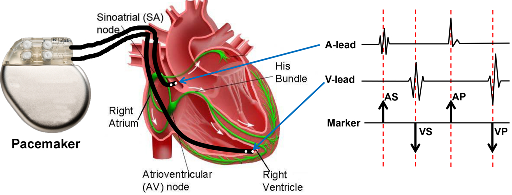
\includegraphics[width=0.9\textwidth]{figs/egm.pdf}
		
%\vspace{-10pt}
\caption{\small (a) Lead placement for a dual chamber pacemaker. (b) Electrogram (EGM) signals measured from pacemaker leads and corresponding internal pacemaker events}
\label{fig:probes}
%\vspace{-15pt}
\end{figure} 

%Implantable pacemakers follow the principle of EP testing. For a dual chamber pacemaker, two leads are inserted into the right atrium and right ventricle, respectively. The pacemaker senses the intrinsic generation and conduction of the electrical signals in the two chambers and deliver electrical pacing when the heart rate and/or atria-to-ventricles conduction interval are abnormal.
The implantable cardiac pacemakers are rhythm management devices designed to treat bradycardia. A typical dual chamber pacemaker has two leads inserted into the heart through the veins which can measure the local electrical activity of the right atrium and right ventricle respectively (\figref{probes}.a). According to the timing between sensed impulses, the pacemaker may deliver electrical pacing to the corresponding chamber to maintain proper heart rhythm.

\section{A Dual Chamber Pacemaker Specification}
The focus of this section is implantable pacemaker, which is one of the simpler implantable cardiac devices.
%The functionality of a pacemaker is based on the timing and patterns of local electrical events. 
The specifications are based on the algorithm descriptions from Boston Scientific manuals (\cite{compass}) and the functional description released as part of the Pacemaker Challenge (\cite{challenge}). 


The pacemaker is designed for patients with bradycardia (i.e. slow heart rate). 
Two leads, one in the right atrium and one in the right ventricle, are inserted into the heart and fixed onto the inner wall of the heart. 
These two leads monitors the local activation of the atria and the ventricles, and generate corresponding sensed events \textsf{(AS, VS)} to its software. 
The software determines the heart condition by measuring time difference between events and delivers pacing events \textsf{(AP, VP)} to the analog circuit when necessary. 
The analog circuit then delivers pacing signals to the heart to maintain heart rate and A-V synchrony. 
In order to deal with different heart condition, pacemakers are able to operate in different modes. 
The modes are labeled using a three character system (e.g. $xyz$). 
The first position describes the pacing locations, the second location describes the sensing locations, and the third position describes how the pacemaker software responds to sensing. 
Here we introduce the widely used DDD mode pacemaker which is a dual chamber mode with sensing and pacing in both atrium and ventricle. 

\begin{figure}[!b]
\center
%\vspace{-10pt}
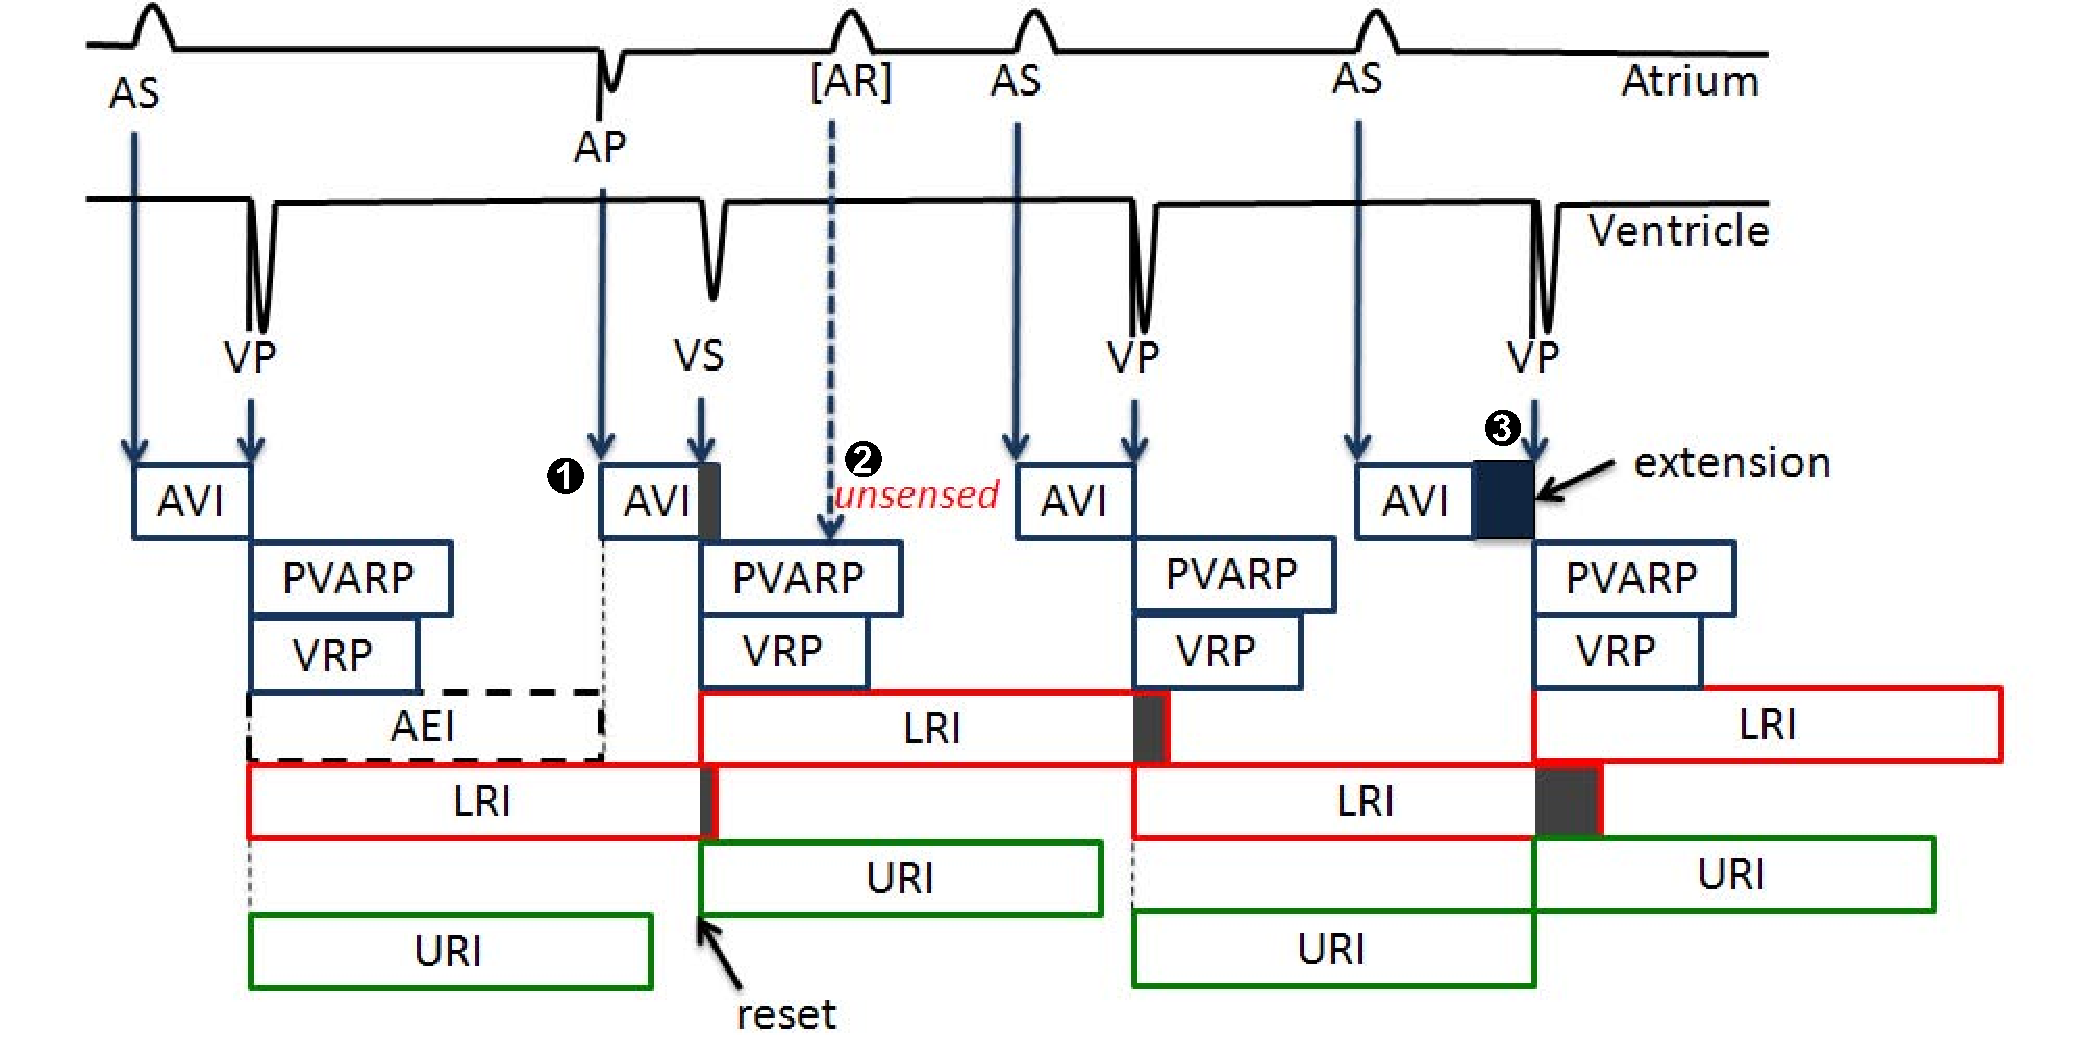
\includegraphics[width=0.85\textwidth]{figs/PM_timers.pdf}
%\vspace{-10pt}
\caption{Basic 5 timing cycles for a dual chamber pacemaker which include the Lower Rate Interval (LRI),  Atrio-Ventricular Interval (AVI), and Upper Rate Interval (URI). Also included are the blanking intervals, Post Ventricular Atrial Refractory Period (PVARP) and Ventricular Refractory Period (VRP), to inhabit action by the pacemaker.}
\label{fig:PMtimers}
%\vspace{-10pt}t

\end{figure} 
A DDD pacemaker has five basic timing cycles triggered by external and internal events, as shown in \figref{PMtimers}. 

\subsubsection{Lower Rate Interval (LRI)}
%\vspace{-5pt}
The Lower Rate Interval (LRI) defines the longest interval allowed between two ventricular events, thus keeping the heart rate above a minimum value. 
In DDD mode, the LRI interval is divided into a V-A interval (TLRI-TAVI) and a A-V interval (TAVI). 
Since the last ventricular event \textsf{(VS, VP)}, if no atrial event has been sensed \textsf{(AS)}, the pacemaker will deliver atrial pacing \textsf{(AP)} after TLRI-TAVI. (Marker 1 in \figref{PMtimers})

%\vspace{-5pt}
\subsubsection{Atrio-Ventricular Interval (AVI) and Upper Rate Interval (URI)}
%\vspace{-5pt}
The function of the AVI timer defines the longest interval between an atrial event and a ventricular event. 
If there is no ventricular event \textsf{(VS)} within TAVI after an atrial event \textsf{(AS, AP)}, and the time since the last ventricular event \textsf{(VS, VP)} is longer than TURI, the pacemaker will deliver ventricular pacing \textsf{(VP)}. (Marker 3 in \figref{PMtimers})
The URI limits the ventricular pacing rate by enforcing a lower bound on the times between consecutive ventricle events. %The UPPAAL design of AVI component is shown in 

%\vspace{-10pt}
\subsection{Post Ventricular Atrial Refractory Period (PVARP) and Post Ventricular Atrial Blanking (PVAB)}
%\vspace{-5pt}
Ventricular events, especially Ventricular Pace \textsf{(VP)} are sometimes so strong that the atrial lead can sense the activation as well. 
This signal may be falsely recognized as an atrial event and disrupt normal pacemaker function. 
This scenario is called crosstalk and was discussed in our previous work (\cite{vhm_embc11}). 
In order to prevent this undesired behavior, and filter potential noises, there is a blanking period (PVAB) followed by a refractory period (PVARP) for the atrial events after each ventricular event \textsf{(VS, VP)}. 
Atrial events during PVAB are ignored and atrial events during PVARP trigger \textsf{AR!} events which can be used in some advanced diagnostic algorithms. (Marker 2 in \figref{PMtimers})

%\vspace{-10pt}
\subsection{Ventricular Refractory Period (VRP)}
%\vspace{-5pt}
The VRP follows each ventricular event \textsf{(VP, VS)} to filter noise and early events in the ventricular channel which could otherwise cause undesired pacemaker behavior. 

\section{Identify Hazards in the Dual Chamber Pacemaker Design}
Implantable pacemakers are designed to treat bradycardia by increasing the heart rate with external pacing. 
Therefore the heart rate should not only be 1) increased to the minimum physiological need, but also 2) should not be increased beyond physiological need. 
Failing to satisfy the two requirements leads to failures that may be harmful to the patient.
Fault tree analysis (FTA) is a top down and deductive failure analysis in which an undesired state of a system is analyzed using Boolean logic to combine a series of lower-level events.
\figref{risk_req} demonstrates two FTAs for two failures corresponding to the two requirements. 
In this section we introduce two well-studied safety hazards in a basic dual chamber pacemaker design.
\begin{figure}[!t]
		\centering
		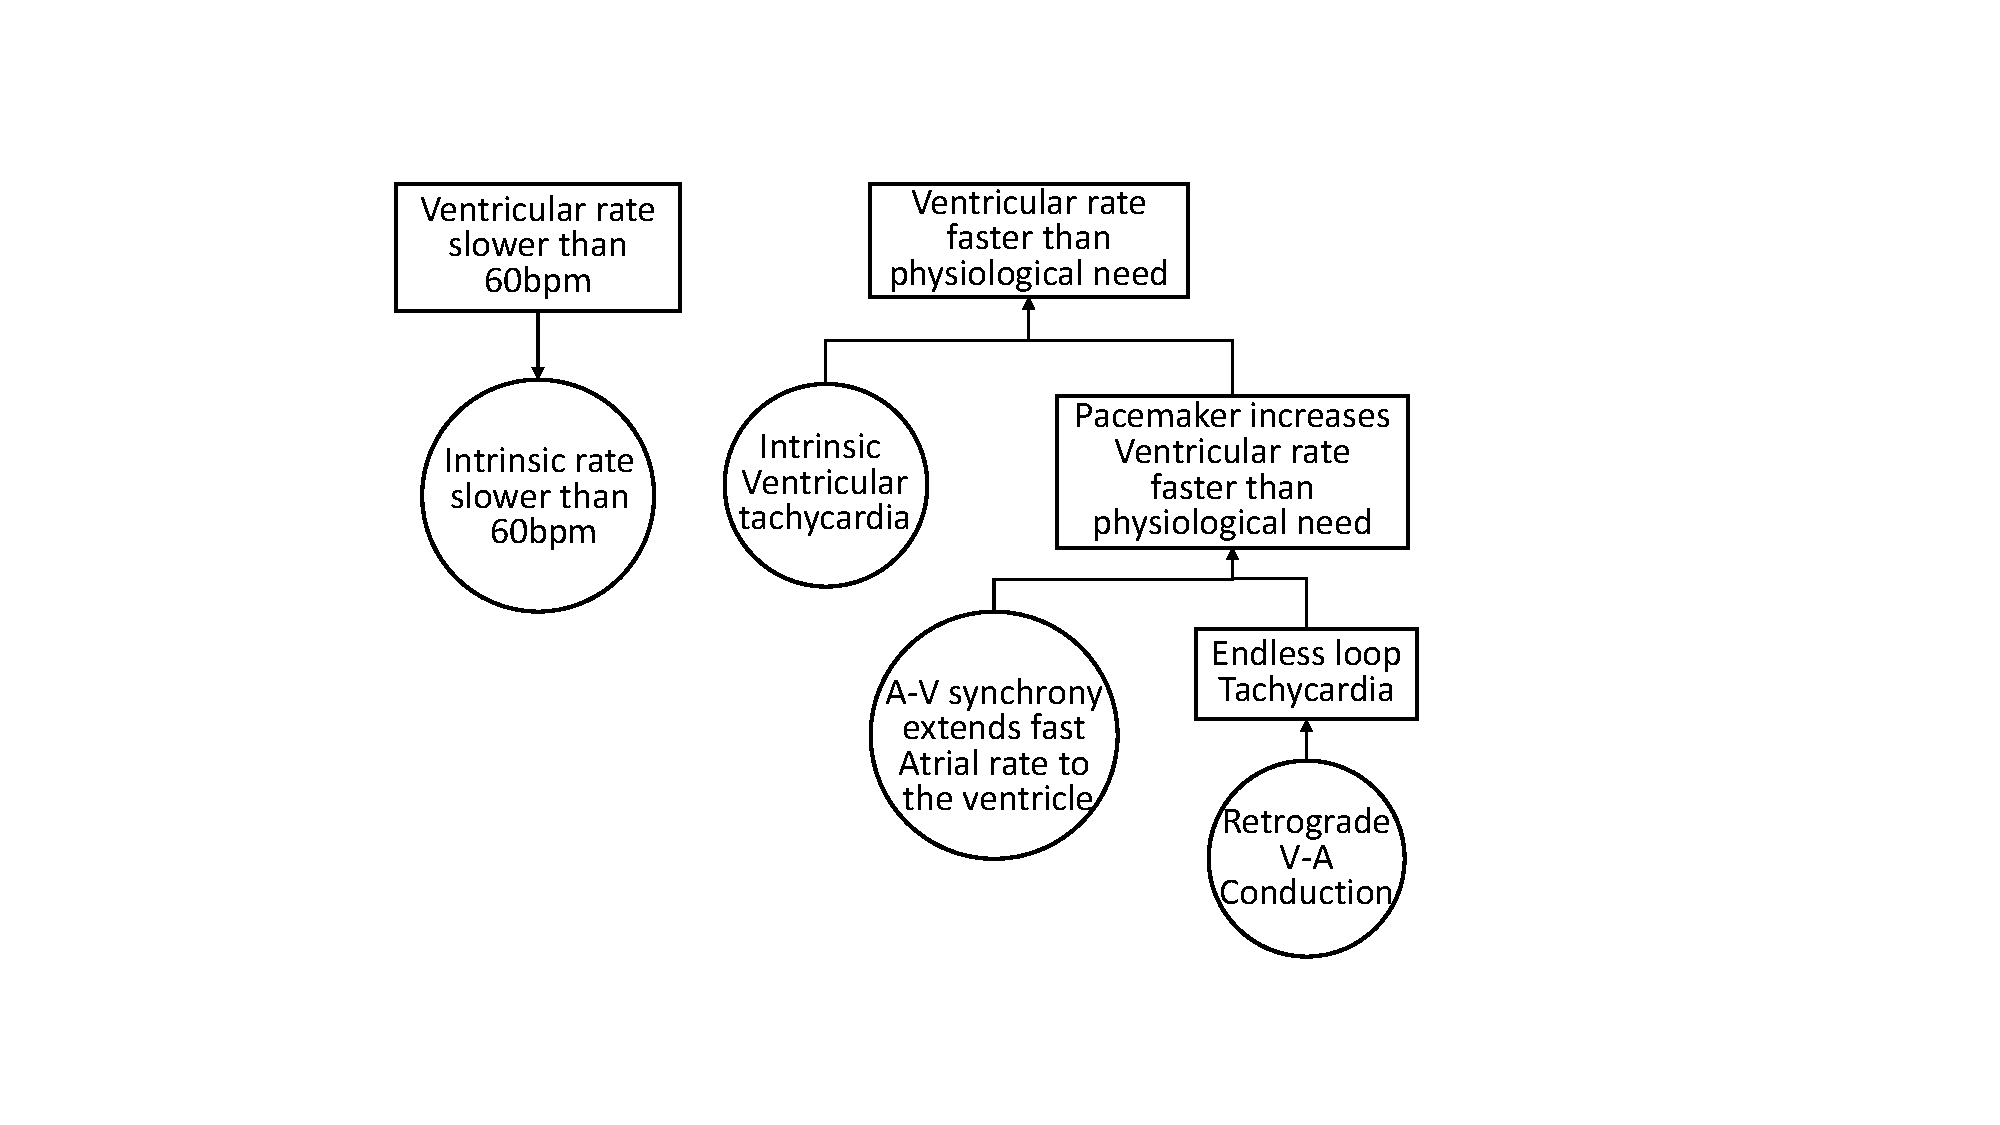
\includegraphics[width=0.8\textwidth]{figs/risk_requirements.pdf}
		\caption{\small Fault Tree Analysis (FTA) for two failures of a pacemaker}
		  %\vspace{-15pt}
		\label{fig:risk_req}
\end{figure}


\subsection{Endless-Loop Tachycardia}
\begin{figure*}
\centering
%		\vspace{-10pt}
		\subfigure [Virtual circuit formed by the pacemaker and the heart] {
				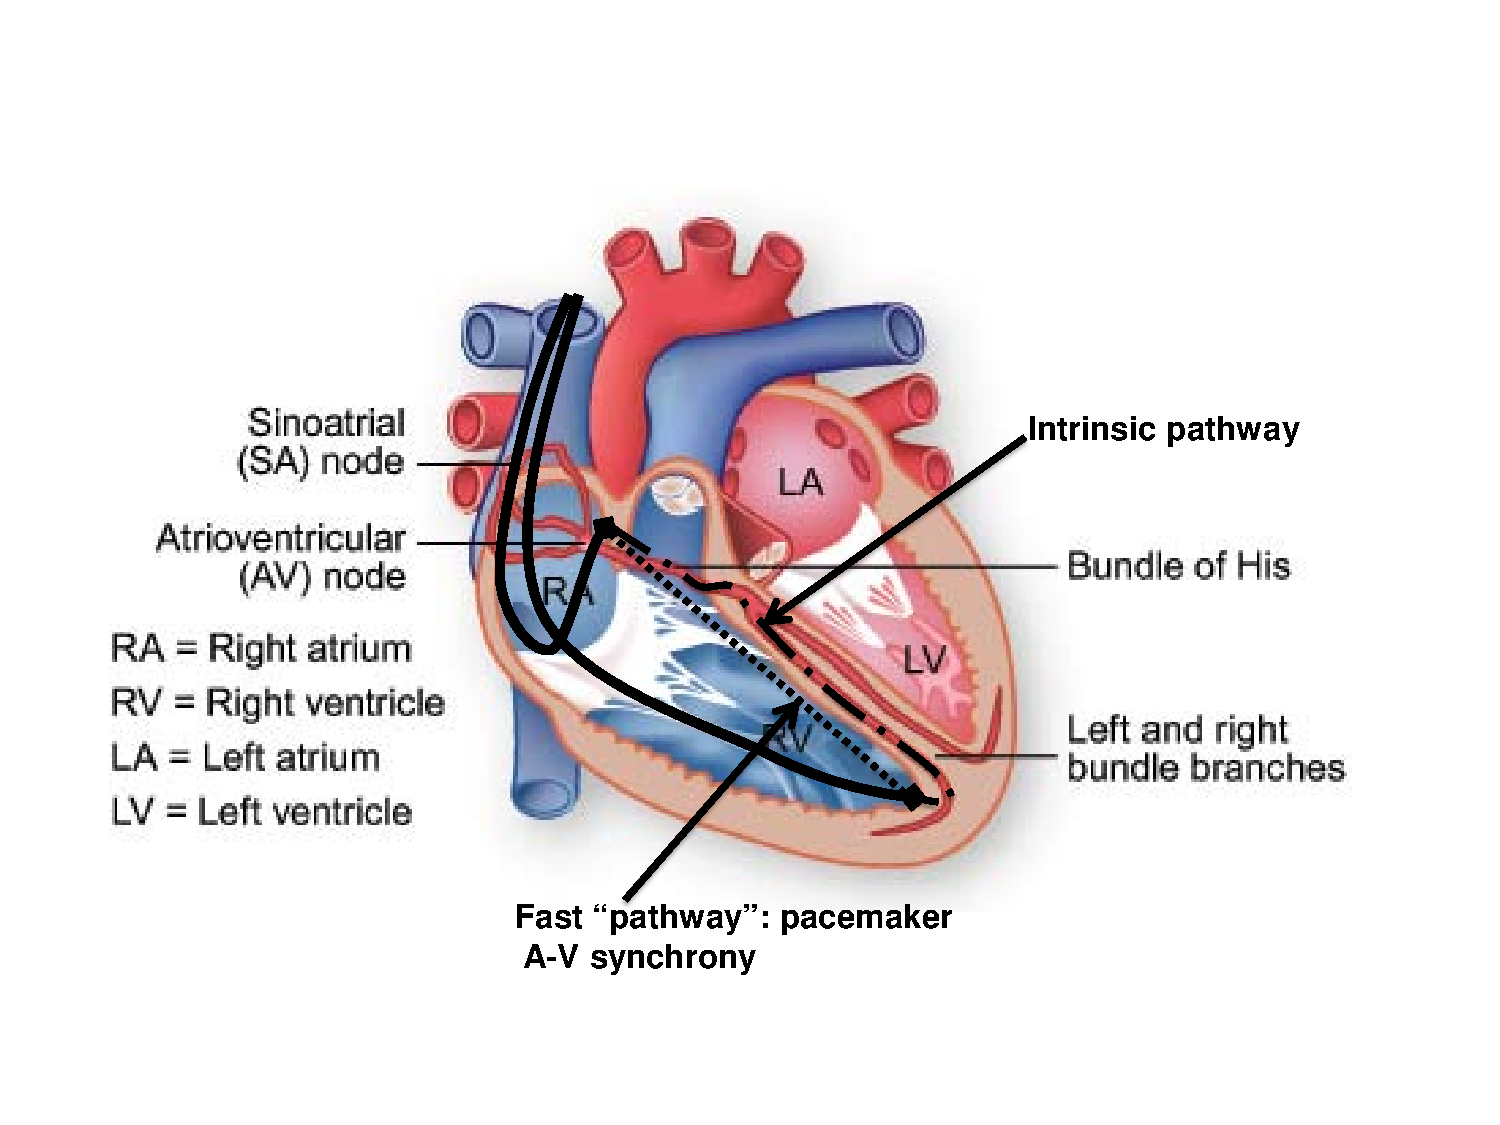
\includegraphics[width=0.45\textwidth]{figs/ELT_str.pdf}
				\label{fig:ELT_demo}
		} 
		\subfigure [Pacemaker trace for ELT initialized by a early ventricular signal]{	
			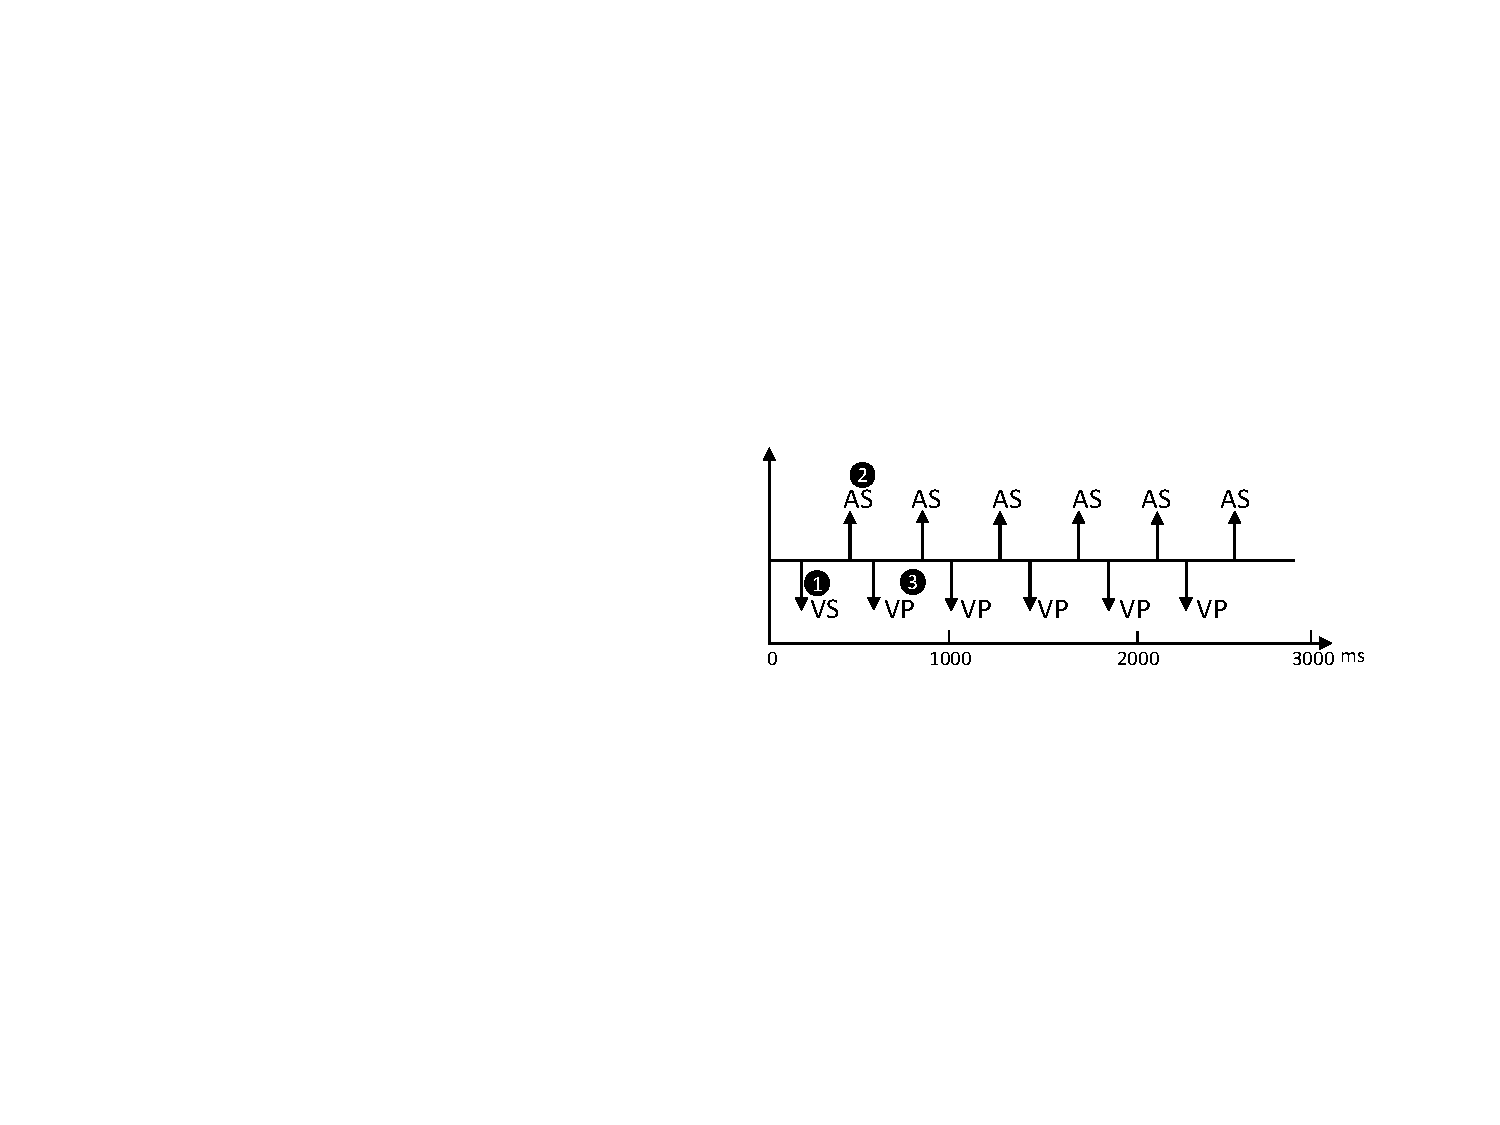
\includegraphics[width=0.45\textwidth]{figs/ELT.pdf}
			\label{fig:ELT}
		}
%		\vspace{-10pt}
	\caption{Endless Loop Tachycardia case study demonstrating the situation when the pacemaker drives the heart into an unsafe state (\cite{vhm_iccps11})}
%\vspace{-15pt}
\end{figure*}

As introduced in the last section, a dual-chamber pacemaker paces the ventricle if no ventricular events are sensed after TAVI, which is equivalent to a virtual atria-to-ventricles conduction pathway. 
This forms a timing loop with the intrinsic (physiological) A-V conduction pathway (see \figref{ELT_demo}). 
A Premature Ventricular Contraction (PVC), i.e. an early extra beat in the ventricles, may trigger another ventricular event (VS) and initiate a V-A conduction through the intrinsic pathway (Marker 1 in \figref{ELT}). 
The pacemaker registers this signal as an Atrial Sense (AS) (Marker 2 in \figref{ELT}). 
A ventricular pace (VP) is delivered after TAVI, as if the signal conducts through the ``virtual" A-V pathway (Marker 3 in \figref{ELT}). 
The VP will trigger another V-A conduction and this VP-AS-VP-AS looping behavior will continue (see \figref{ELT}). 
The interval between atrial events is TAVI plus the V-A conduction delay, which is normally shorter than the delay between intrinsic heart beats, thus driving the ventricular rate as high as the Upper Rate Limit. 
During ELT, the heart rate is not only high, but also fixed without changing according to physiological need, which is an unsafe scenario.

\subsection{Atrial Tachycardia Response}

Supraventricular Tachycardia (SVT) is an arrhythmia with an abnormally fast atrial rate. %\figref{SVT} is a series of simulation results for closed-loop interaction between a heart model with SVT and the pacemaker model. The atrial and ventricular channels show electrogram inputs to the pacemaker and the pacemaker channel shows the corresponding events received and generated by the pacemaker software, \cite{vhm_embc11}.
Typically, in a heart without pacemaker, the AV node, which has a long refractory period, can filter most of the fast atrial activations during SVT, thus the ventricular rate remains relatively normal. \figref{SVT_none} demonstrates a pacemaker event trace during SVT, with a pacemaker in ODO mode, which just sensing in both channels. 
As there is no pacing in ODO mode, the heart is in open-loop with the pacemaker. In this particular case, every 3 atrial events (AS) correspond to 1 ventricular event (VS) during SVT. 
As an arrhythmia, SVT is still considered a safe heart condition since the ventricles operate under normal rate and still maintain adequate cardiac output. 

However, in the closed loop case with the DDD pacemaker, the AVI component of a dual chamber pacemaker is equivalent to a virtual pathway in parallel to the intrinsic conduction pathway between the atria and the ventricles. The pacemaker tries to maintain 1:1 A-V conduction and thus increases the ventricular rate inappropriately to match the atrial rate.  This is known as Pacemaker Mediated Tachycardia (PMT) as the heart would have been safe without the pacemaker and its virtual pathway. \figref{SVT_DDD} shows the pacemaker trace of the same SVT case with DDD pacemaker. Although half of the fast atrial events are filtered by the PVARP period ([AR]s), the DDD pacemaker still drives the closed-loop system into 2:1 A-V conduction with faster ventricular rate. Maintaining A-V delay is less important than maintaining an appropriate ventricular rate. The DDD pacemaker violates a higher priority requirement in order to satisfy a lower priority requirement, which is inappropriate.
\begin{figure*}[!t]
\centering
		\subfigure [\small]{			
		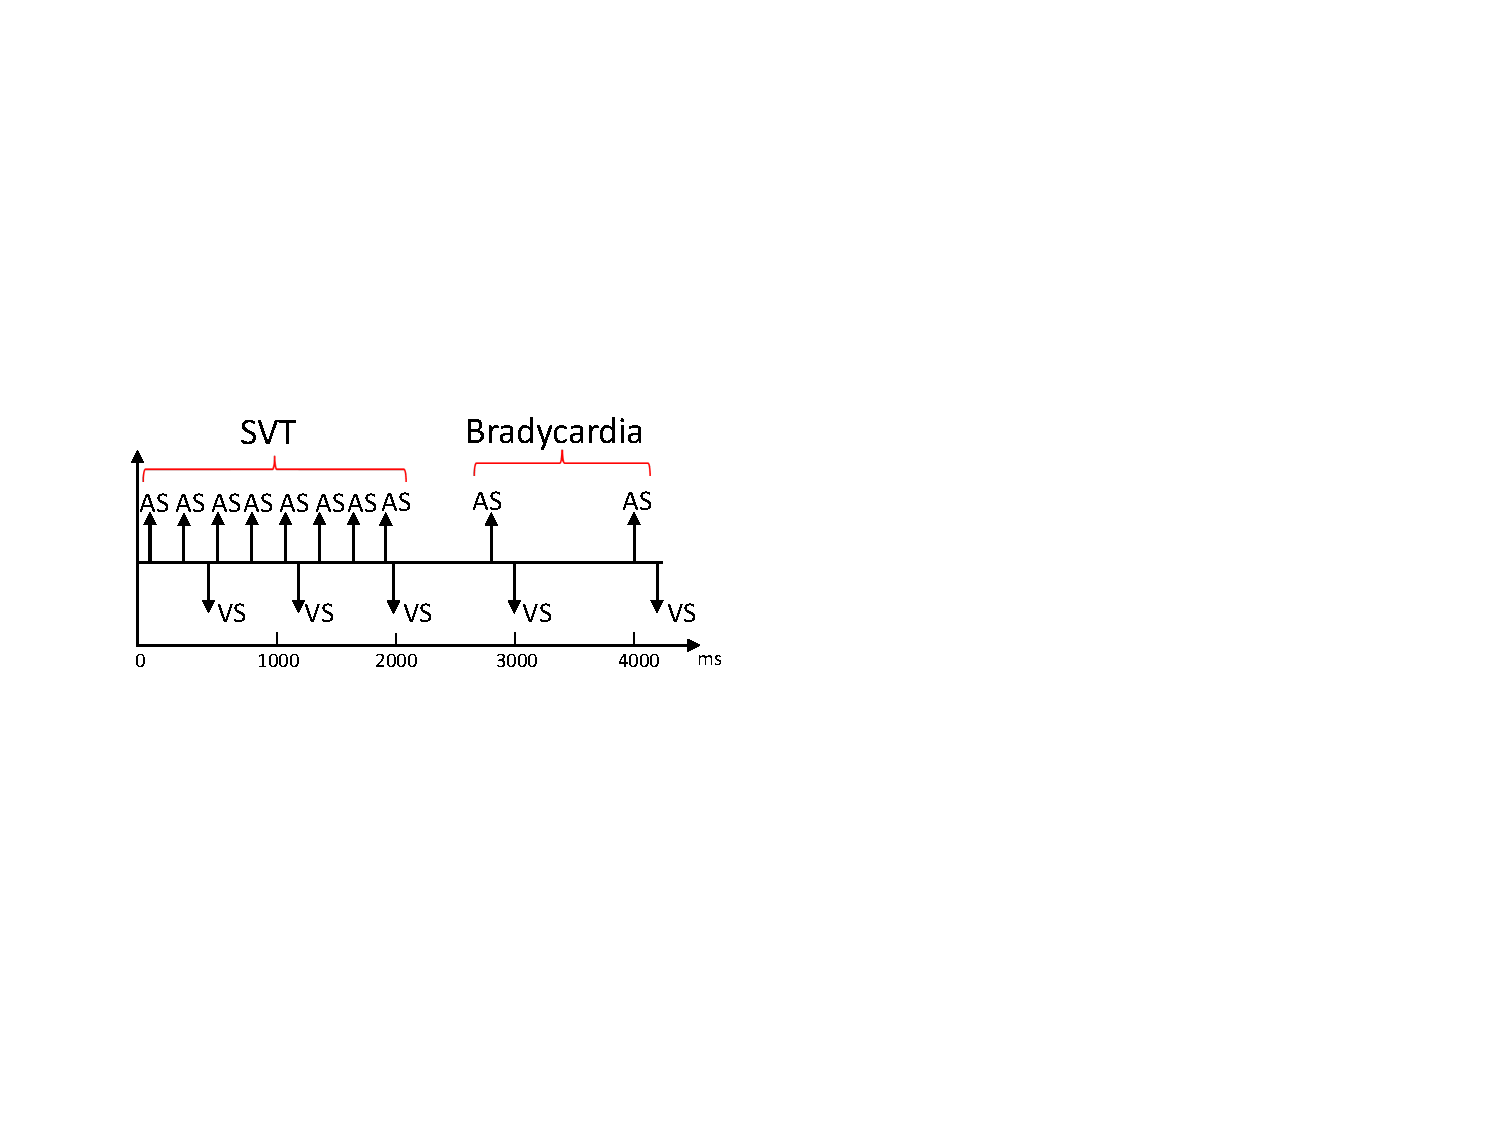
\includegraphics[width=0.45  \textwidth]{figs/SVT_none.pdf}
		\label{fig:SVT_none}
		} 
%	\hspace{.1in}%
		
		\subfigure [\small] 
		{
		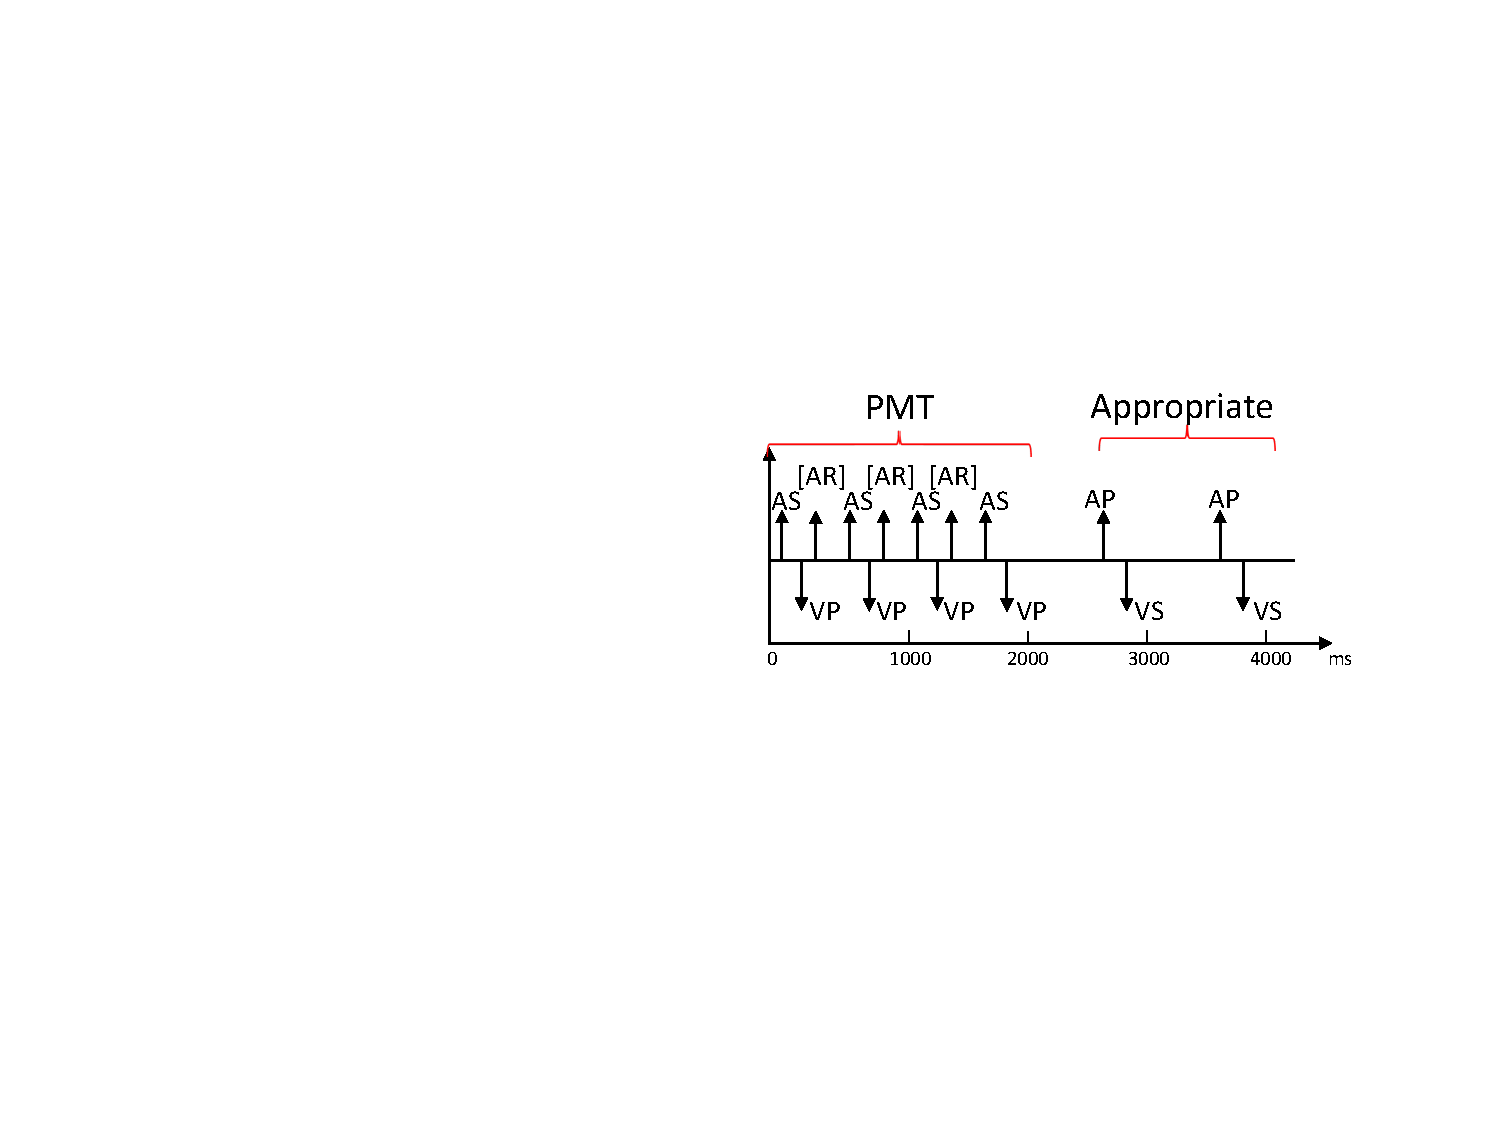
\includegraphics[width=0.45\textwidth]{figs/SVT_DDD.pdf}
		\label{fig:SVT_DDD}
		} 
\caption{\small Benign open loop case: SVT without a pacemaker or with a pacemaker in sense-only mode (ODO) (b) Dangerous closed-loop-case SVT with DDD pacemaker which tries to match the fast atrial rate with a corresponding (and dangerous) fast ventricular rate.}
\end{figure*} 

\section{Discussion}
Implantable cardiac devices such as implantable pacemakers are typical autonomous medical devices.
Despite their seemingly simple controllers, the pacemakers also subject to the three challenges discussed in Chapter 1:
\begin{itemize}
	\item The physiology of the heart and its interaction with the rest of the body are complex.
\item The pacemakers have to safely operate within a large variety of physiological conditions.
\item A dual chamber pacemaker can only observe electrical activities from two local sites in the heart.
\end{itemize}
In the remaining dissertation, I will demonstrate the application of physiological models in various model-based techniques to provide safety and efficacy confidence to the pacemaker design.


